% Review II presentation -- built on template_presentation.tex (kept unchanged).
% Compile with: pdflatex r2_presentation.tex  (run twice)
%
% RULE FOR THIS DECK: Modules 4, 5 and 6 are NOT built. The transformer,
% meta-learning, comorbidity fusion and Bayesian classifier are DESIGN only.
% No accuracy, AUC, ROC, confusion matrix, calibration or attention result
% exists, and none may be shown or implied.
%
% Structure: slides 2-12 explain the project for a reader who has not seen it
% (reusing the Review I material); slides 13-25 are the Review II content;
% backup slides follow "Thank You" and are not counted in the page numbers:
% glossary, data limitations, residual motion and site effects, the 246-ROI
% verification pair and "why 246 regions", technology stack, the Phase 2
% (modelling) details (design only) and, last, the First Review queries and
% answers.
% Every figure in figures/ is made by a make_*.py script in that folder from
% real project outputs.

\documentclass[aspectratio=169,11pt]{beamer}

% ---------- Theme and colours (unchanged from the template) ----------
\usetheme{Madrid}
\usecolortheme{default}
\definecolor{UniversityBlue}{RGB}{16,62,110}
\definecolor{AccentBlue}{RGB}{30,136,229}
\definecolor{LightBlue}{RGB}{232,242,252}
\definecolor{DarkGray}{RGB}{55,65,81}

\setbeamercolor{structure}{fg=UniversityBlue}
\setbeamercolor{palette primary}{bg=UniversityBlue,fg=white}
\setbeamercolor{palette secondary}{bg=AccentBlue,fg=white}
\setbeamercolor{frametitle}{bg=UniversityBlue,fg=white}
\setbeamercolor{block title}{bg=UniversityBlue,fg=white}
\setbeamercolor{block body}{bg=LightBlue,fg=black}
\setbeamercolor{alerted text}{fg=AccentBlue}

% ---------- Packages ----------
\usepackage[T1]{fontenc}
\usepackage[utf8]{inputenc}
\usepackage{lmodern}
\usepackage{graphicx}
\usepackage{booktabs}
\usepackage{array}
\usepackage{tabularx}
\usepackage{tikz}
\usetikzlibrary{positioning}
\usepackage{amsmath}
\usepackage{listings}
\usepackage{xcolor}
\usepackage{colortbl}
\usepackage{hyperref}
\usepackage{pgfgantt}   % plan-versus-actual timeline (not in the template)
\usepackage{multicol}   % two-column reference list (not in the template)
\usepackage{appendixnumberbeamer}  % backup slides are not counted in the total

% ---------- General settings ----------
\setbeamertemplate{navigation symbols}{}
\setbeamertemplate{caption}[numbered]
\setbeamertemplate{itemize item}{\color{AccentBlue}$\blacktriangleright$}
\setbeamertemplate{itemize subitem}{\color{UniversityBlue}$\bullet$}
\setbeamersize{text margin left=0.7cm,text margin right=0.7cm}

% Footer: project title, institution and slide number
\setbeamertemplate{footline}{%
  \leavevmode%
  \hbox{%
    \begin{beamercolorbox}[wd=.42\paperwidth,ht=2.7ex,dp=1.1ex,leftskip=.6em]{author in head/foot}%
      \insertshorttitle
    \end{beamercolorbox}%
    \begin{beamercolorbox}[wd=.46\paperwidth,ht=2.7ex,dp=1.1ex,center]{date in head/foot}%
      Department of Computer Science and Engineering
    \end{beamercolorbox}%
    \begin{beamercolorbox}[wd=.12\paperwidth,ht=2.7ex,dp=1.1ex,center]{page number in head/foot}%
      \insertframenumber/\inserttotalframenumber
    \end{beamercolorbox}%
  }%
  \vskip0pt%
}

% ---------- Code style ----------
\lstset{
  basicstyle=\ttfamily\scriptsize,
  keywordstyle=\color{UniversityBlue}\bfseries,
  commentstyle=\color{gray},
  stringstyle=\color{AccentBlue},
  numbers=none,
  frame=single,
  breaklines=true,
  showstringspaces=false
}

% ---------- Status colours (added; theme colours untouched) ----------
\definecolor{DoneGreen}{RGB}{27,122,61}
\definecolor{PartAmber}{RGB}{176,110,0}
\definecolor{NotGray}{RGB}{110,110,110}
\newcommand{\done}{\textcolor{DoneGreen}{\textbf{Complete}}}
\newcommand{\partly}{\textcolor{PartAmber}{\textbf{Partly}}}
\newcommand{\notst}{\textcolor{NotGray}{\textbf{Not started}}}
\newcommand{\todo}[1]{\textcolor{red}{[#1]}}

% ---------- Editable project details ----------
\title[AD Progression from rs-fMRI]{Assessment of Alzheimer's Disease Progression Using
Comorbidity-Aware Meta-Bayesian Framework with Resting-State fMRI}
\subtitle{Second Review}
\author[Student Team]{%
  Harishkanna R (3122235001302)\\
  Dhananchezhiyan M (3122235001041)\\
  Nagindhar Sachein R L (3122235001702)
}
\institute[SSN]{%
  Guided by: Dr. N. Ahana Priyanka, Assistant Professor\\[2mm]
  Department of Computer Science and Engineering\\
  Sri Sivasubramaniya Nadar College of Engineering
}
\date{Academic Year 2026--2027}

\begin{document}

% =====================================================================
% PART A. UNDERSTANDING THE PROJECT (for a reader new to it)
% =====================================================================

% 1. Title slide
\begin{frame}[plain]
  \titlepage
  \begin{tikzpicture}[remember picture,overlay]
    \node[anchor=south east,xshift=-0.5cm,yshift=0.4cm]
    at (current page.south east){
\includegraphics[width=1.7cm]{ssn-logo.png}};
  \end{tikzpicture}
\end{frame}

% 2. Background and Motivation (Review I, condensed)
\begin{frame}{Background and Motivation}
  \begin{columns}[c,onlytextwidth]
    \column{0.50\textwidth}
      \begin{itemize}
        \item \textbf{Alzheimer's disease (AD)} is the most common cause of dementia,
              about 60--70\% of cases worldwide.
        \item It is \textbf{progressive}: memory, reasoning and daily function decline,
              mostly after age 65.
        \item India's ageing population is making the burden grow.
        \item Tissue loss (right) appears late. \textbf{Brain activity}, measured with
              functional MRI, can change earlier.
      \end{itemize}
    \column{0.48\textwidth}
      \centering
      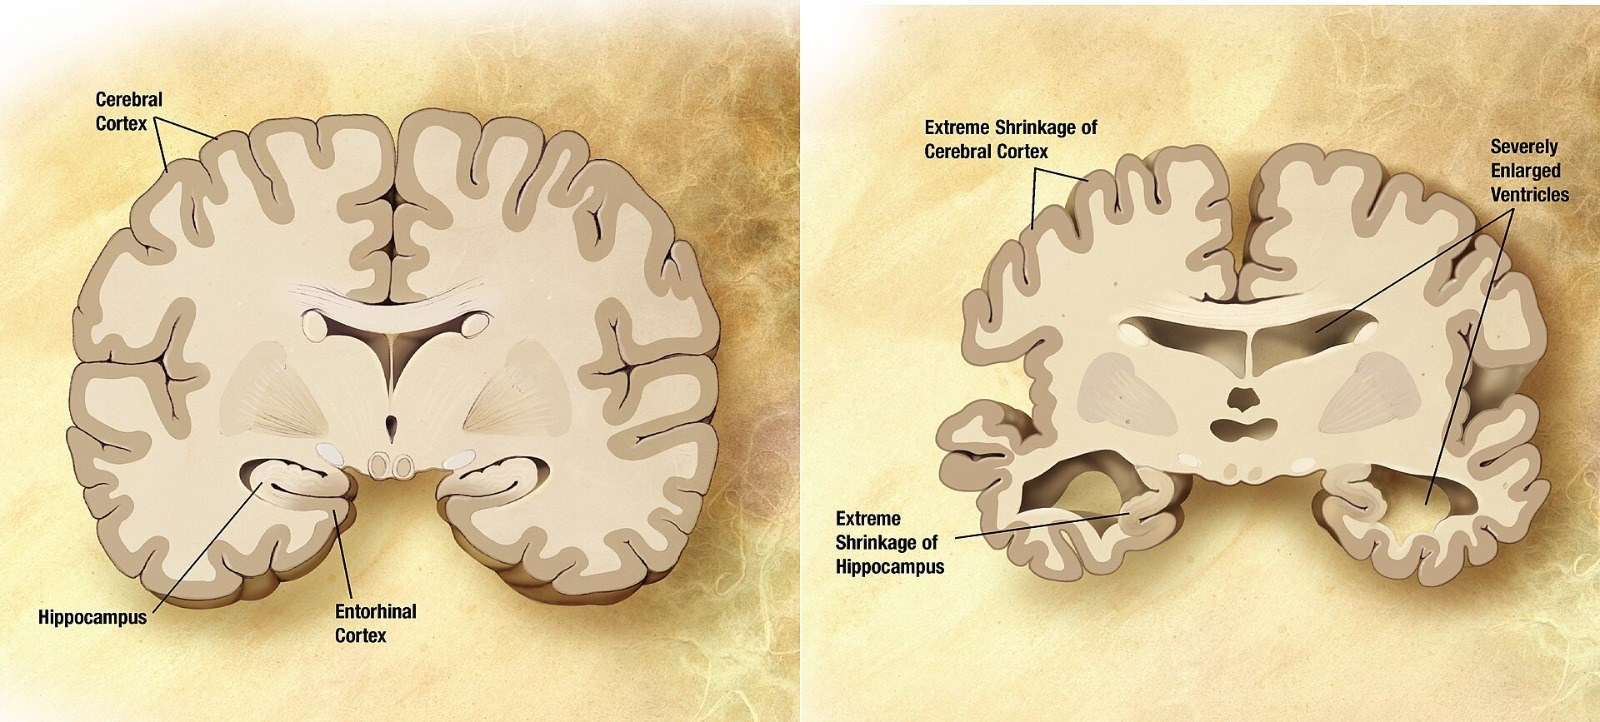
\includegraphics[width=\linewidth]{figures/r1_ad_brain_coronal.jpg}\par
      {\scriptsize Healthy brain (left) and advanced AD (right): thinner cortex, shrunken
      hippocampus, enlarged ventricles. Illustration reused from Review I.}
  \end{columns}
\end{frame}

% 3. The six stages (no counts in the boxes; scan range stated in the text)
\begin{frame}{The Six Stages of Progression}
  \centering
  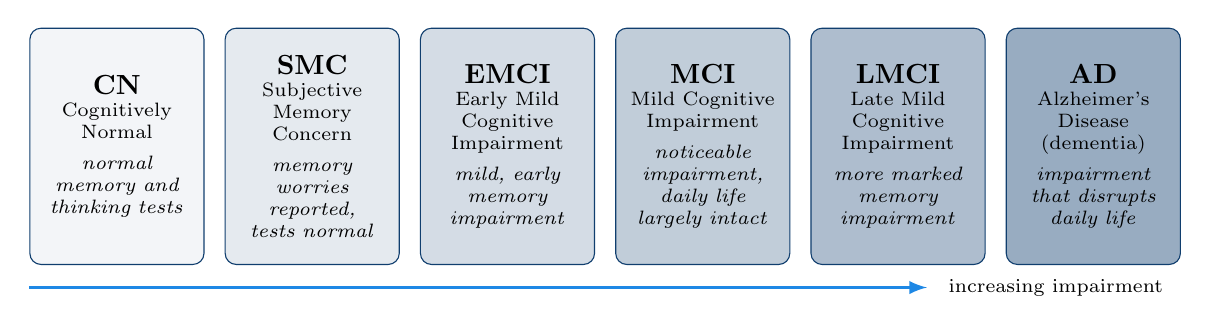
\begin{tikzpicture}[>=latex,
      stg/.style={draw=UniversityBlue,rounded corners,text width=2.0cm,minimum height=3.0cm,
                  align=center,font=\scriptsize,inner sep=3pt,anchor=north west}]
    \node[stg,fill=UniversityBlue!5]  at (0,0)    {{\normalsize\bfseries CN}\\ Cognitively Normal\\[3pt] \emph{normal memory and thinking tests}};
    \node[stg,fill=UniversityBlue!11] at (2.48,0) {{\normalsize\bfseries SMC}\\ Subjective Memory Concern\\[3pt] \emph{memory worries reported, tests normal}};
    \node[stg,fill=UniversityBlue!18] at (4.96,0) {{\normalsize\bfseries EMCI}\\ Early Mild Cognitive Impairment\\[3pt] \emph{mild, early memory impairment}};
    \node[stg,fill=UniversityBlue!26] at (7.44,0) {{\normalsize\bfseries MCI}\\ Mild Cognitive Impairment\\[3pt] \emph{noticeable impairment, daily life largely intact}};
    \node[stg,fill=UniversityBlue!34] at (9.92,0) {{\normalsize\bfseries LMCI}\\ Late Mild Cognitive Impairment\\[3pt] \emph{more marked memory impairment}};
    \node[stg,fill=UniversityBlue!43] at (12.4,0) {{\normalsize\bfseries AD}\\ Alzheimer's Disease (dementia)\\[3pt] \emph{impairment that disrupts daily life}};
    \draw[->,very thick,draw=AccentBlue] (0,-3.3) -- (11.4,-3.3);
    \node[anchor=west,font=\scriptsize] at (11.55,-3.3) {increasing impairment};
  \end{tikzpicture}
  \vspace{0.2cm}

  \begin{itemize}
    \item Labels are ADNI's diagnostic groups. Each stage has \textbf{about 30 scans}.
    \item The model treats the stages as an \textbf{ordered scale} (fixed at Review I):
          CN $\rightarrow$ SMC $\rightarrow$ EMCI $\rightarrow$ MCI $\rightarrow$ LMCI $\rightarrow$ AD.
    \item Neighbouring stages overlap, so every label should come with a \textbf{confidence}.
  \end{itemize}
\end{frame}

% 4. Problem Statement
\begin{frame}{Problem Statement}
  \begin{alertblock}{Problem}
    Existing systems analyse rs-fMRI biomarkers \textbf{independently} and omit clinical
    context, giving \textbf{overconfident, deterministic staging errors} on borderline subjects.
  \end{alertblock}
  \vspace{0.2cm}
  \begin{itemize}
    \item \textbf{Context:} dementia progresses through six ordered stages.
    \item \textbf{Limitation:} pipelines isolate ALFF, ReHo, DC and FC.
    \item \textbf{Clinical gap:} models ignore how comorbidities modify neurodegeneration.
  \end{itemize}
  \begin{block}{Research question}
    Can a common AD progression representation be found across several functional
    biomarkers, accounting for comorbidity and prediction uncertainty?
  \end{block}
\end{frame}

% 5. Proposed System Architecture (replaces the earlier one-picture overview)
\begin{frame}{Proposed System Architecture}
  \centering
  \resizebox{0.98\textwidth}{!}{%
  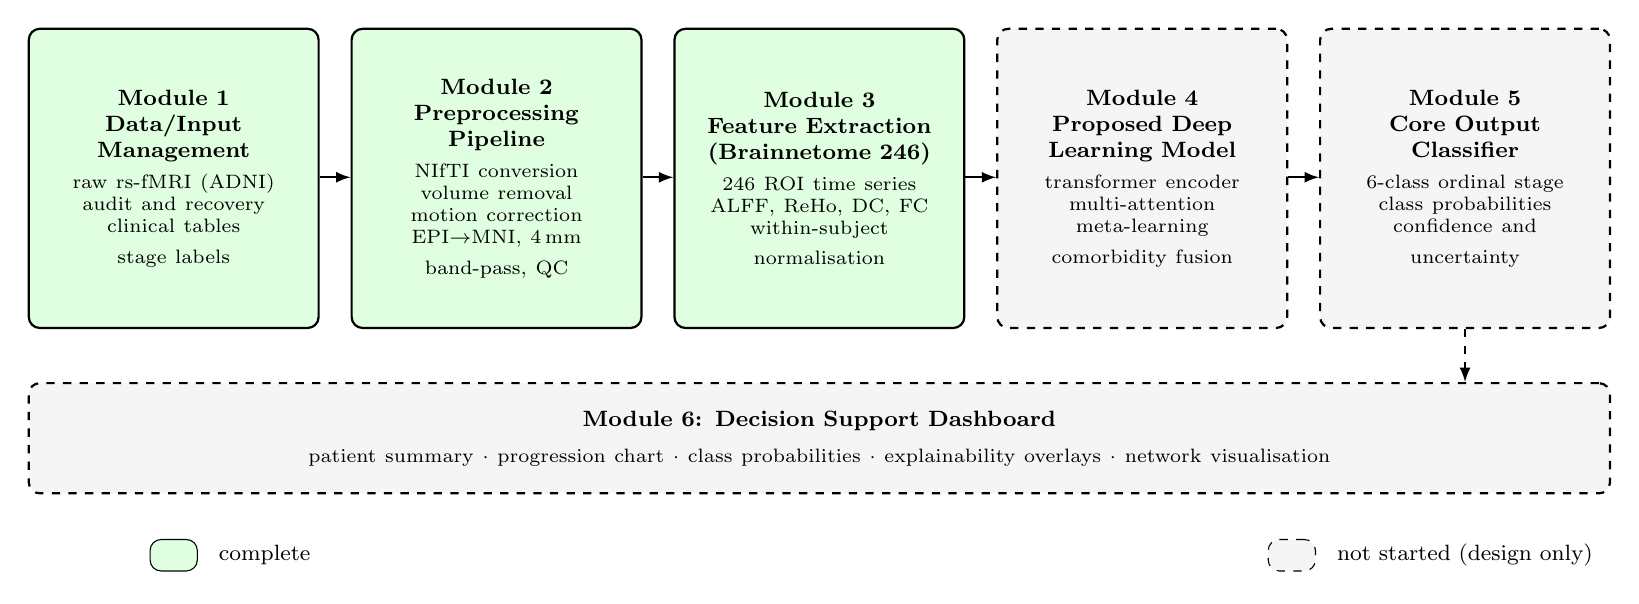
\begin{tikzpicture}[font=\small,>=latex]
    \tikzset{
      mod/.style={rounded corners,thick,draw,align=center,text width=3.4cm,
                  minimum height=3.8cm,inner sep=4pt,anchor=north,
                  execute at begin node={\hyphenpenalty=10000\exhyphenpenalty=10000}},
      dn/.style={mod,fill=green!12},
            pl/.style={mod,dashed,fill=gray!8},
      ar/.style={->,thick}}
    \node[dn] (m1) at (0,0)    {\footnotesize\textbf{Module 1}\\\footnotesize\textbf{Data/Input}\\\footnotesize\textbf{Management}\\[3pt]\scriptsize raw rs-fMRI (ADNI)\\ audit and recovery\\ clinical tables\\ stage labels};
    \node[dn] (m2) at (4.1,0)  {\footnotesize\textbf{Module 2}\\\footnotesize\textbf{Preprocessing}\\\footnotesize\textbf{Pipeline}\\[3pt]\scriptsize NIfTI conversion\\ volume removal\\ motion correction\\ EPI$\rightarrow$MNI, 4\,mm\\ band-pass, QC};
    \node[dn] (m3) at (8.2,0)  {\footnotesize\textbf{Module 3}\\\footnotesize\textbf{Feature Extraction}\\\footnotesize\textbf{(Brainnetome 246)}\\[3pt]\scriptsize 246 ROI time series\\ ALFF, ReHo, DC, FC\\ within-subject\\ normalisation};
    \node[pl] (m4) at (12.3,0) {\footnotesize\textbf{Module 4}\\\footnotesize\textbf{Proposed Deep}\\\footnotesize\textbf{Learning Model}\\[3pt]\scriptsize transformer encoder\\ multi-attention\\ meta-learning\\ comorbidity fusion};
    \node[pl] (m5) at (16.4,0) {\footnotesize\textbf{Module 5}\\\footnotesize\textbf{Core Output}\\\footnotesize\textbf{Classifier}\\[3pt]\scriptsize 6-class ordinal stage\\ class probabilities\\ confidence and\\ uncertainty};
    \node[pl,anchor=north,minimum height=1.4cm,text width=19.8cm] (m6) at (8.2,-4.5) {\footnotesize\textbf{Module 6: Decision Support Dashboard}\\[2pt]\scriptsize patient summary $\cdot$ progression chart $\cdot$ class probabilities $\cdot$ explainability overlays $\cdot$ network visualisation};
    \foreach \a/\b in {m1/m2,m2/m3,m3/m4,m4/m5} \draw[ar] (\a.east |- 0,-1.9) -- (\b.west |- 0,-1.9);
    \draw[ar,dashed] (m5.south) -- (m5.south |- m6.north);
    \node[draw,fill=green!12,rounded corners,minimum width=0.6cm,minimum height=0.4cm] at (0,-6.7) {};
    \node[anchor=west] at (0.45,-6.7) {\footnotesize complete};
    \node[draw,dashed,fill=gray!8,rounded corners,minimum width=0.6cm,minimum height=0.4cm] at (14.2,-6.7) {};
    \node[anchor=west] at (14.65,-6.7) {\footnotesize not started (design only)};
  \end{tikzpicture}}
  \vspace{0.25cm}

  \small \textbf{Goal:} place each person on the six-stage scale from a resting-state scan and
  clinical context, and say how sure the model is.
\end{frame}

% 6. Resting-state fMRI in plain words
\begin{frame}{Resting-State fMRI in Plain Words}
  \small
  \begin{itemize}
    \item The participant lies still in the scanner and does \textbf{no task}.
    \item Every 3\,s the scanner takes a 3-D picture of the brain: 140 pictures, about 7 minutes.
    \item The signal is \textbf{BOLD}: local blood oxygenation, a proxy for neural activity.
    \item Slow fluctuations (0.01--0.10\,Hz) in linked regions rise and fall together.
  \end{itemize}
  \vspace{0.1cm}
  \begin{columns}[T,onlytextwidth]
    \column{0.45\textwidth}
      \centering
      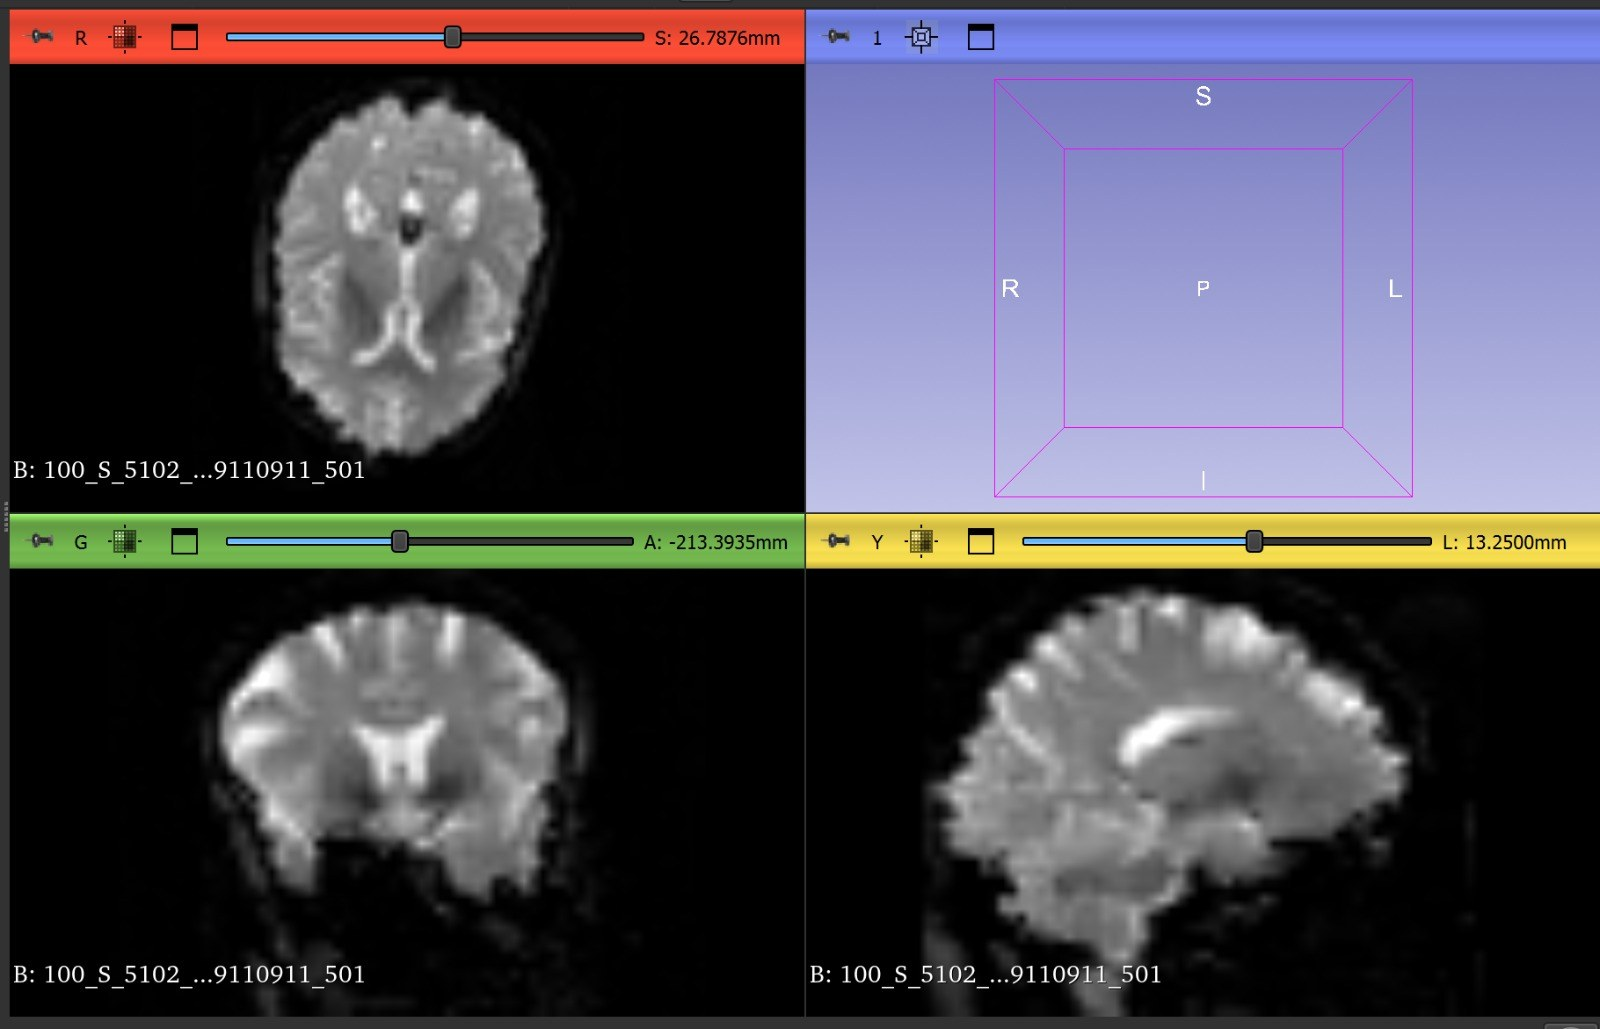
\includegraphics[height=2.85cm]{figures/r1_nifti_viewer.jpg}\par
      {\scriptsize One converted scan in three planes (Review I).}
    \column{0.53\textwidth}
      \centering
      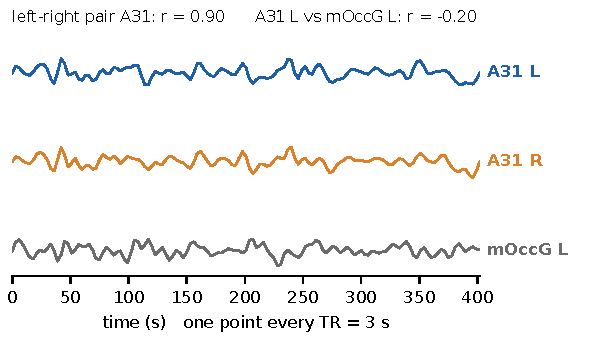
\includegraphics[height=2.85cm]{figures/ts_example.pdf}\par
      {\scriptsize Three regions from one scan: left and right A31 move together, an occipital region does not.}
  \end{columns}
\end{frame}

% 7. The dataset
\begin{frame}{The Dataset: ADNI}
  \begin{columns}[T,onlytextwidth]
    \column{0.52\textwidth}
      \small
      \begin{itemize}
        \item \textbf{ADNI} is a public, multi-site study that shares brain scans and clinical
              data \cite{r1,r2}.
        \item We use its \textbf{resting-state fMRI only}: the download has no structural (T1) scans.
        \item Each scan: 140 volumes, TR = 3\,s for most, voxels of about 3\,mm.
        \item 175 scans audited, 2 excluded (1 duplicate, 1 truncated): 173 eligible,
              \textbf{165 processed}. Eight failed: their TR of 6.02\,s is too slow for the
              0.01--0.10\,Hz band.
        \item \textbf{Target: 30 scans per stage, 180 in all.} The last column shows the processed scans
              still to add (SMC and MCI are already above 30).
      \end{itemize}
    \column{0.45\textwidth}
      \centering
      \footnotesize
      \begin{tabular}{lrrr}
        \toprule
        \textbf{Stage} & \textbf{Elig.} & \textbf{Proc.} & \textbf{To 30} \\
        \midrule
        CN   & 29 & 27 & +3 \\
        SMC  & 32 & 31 & 0 \\
        EMCI & 30 & 29 & +1 \\
        MCI  & 35 & 32 & 0 \\
        LMCI & 22 & 21 & +9 \\
        AD   & 25 & 25 & +5 \\
        \midrule
        \textbf{Total} & \textbf{173} & \textbf{165} & \textbf{+18} \\
        \bottomrule
      \end{tabular}\par
      \vspace{0.2cm}
      {\scriptsize Counts are per scan. Elig.: passed the audit; Proc.: preprocessed;
      To 30: processed scans still to add for 30 per stage.}
  \end{columns}
\end{frame}

% 8. Clinical context
\begin{frame}{Clinical Context: Covariates and Comorbidity}
  \small
  \renewcommand{\arraystretch}{1.3}
  \begin{tabularx}{\textwidth}{>{\bfseries\raggedright\arraybackslash}p{4.4cm}>{\raggedright\arraybackslash}X}
    \toprule
    Covariate & What it is, and why it matters \\
    \midrule
    Age & years at the scan; risk rises with age \\
    APOE $\varepsilon$4 & copies of the $\varepsilon$4 variant; strongest common genetic risk factor \\
    MMSE & 0--30 cognitive screening score; lower is worse \\
    CDR-SB & 0--18 clinician-rated severity; higher is worse \\
    GDS & 0--15 depression scale; often accompanies decline \\
    Cardiovascular history & ADNI category MH4CARD; includes hypertension \\
    Endocrine/metabolic history & ADNI category MH9ENDO; includes diabetes \\
    \bottomrule
  \end{tabularx}
\end{frame}

% 9. The four biomarkers (plain words)
\begin{frame}{The Four Feature Biomarkers}
  \begin{columns}[T,onlytextwidth]
    \column{0.245\textwidth}
      \centering
      {\bfseries ALFF}\\ {\scriptsize how strong}\\[2pt]
      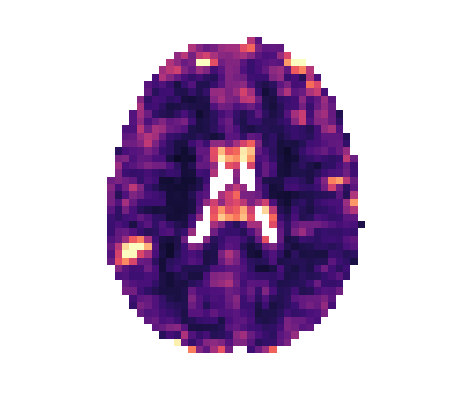
\includegraphics[height=1.75cm]{figures/bm_alff.png}\\[2pt]
      \scriptsize How big the slow swings of a region's signal are.\\ Big swings: stronger activity.
    \column{0.245\textwidth}
      \centering
      {\bfseries ReHo}\\ {\scriptsize how locally in step}\\[2pt]
      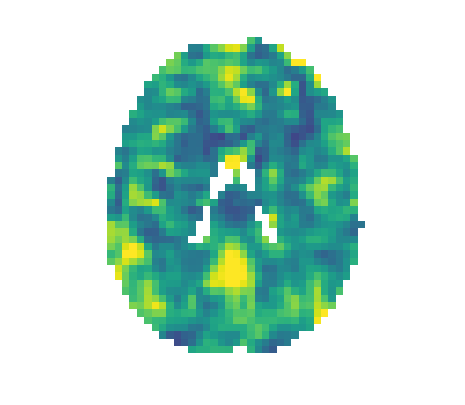
\includegraphics[height=1.75cm]{figures/bm_reho.png}\\[2pt]
      \scriptsize Do the small spots inside a region rise and fall together?\\ Yes: the region works in step.
    \column{0.245\textwidth}
      \centering
      {\bfseries FC}\\ {\scriptsize who talks to whom}\\[2pt]
      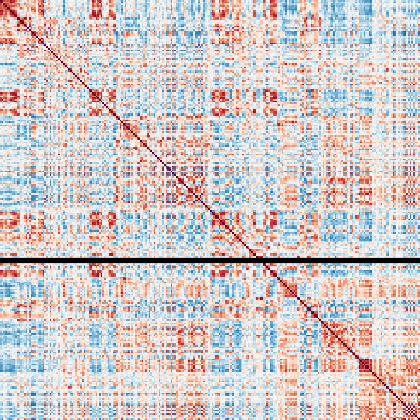
\includegraphics[height=1.75cm]{figures/bm_fc.png}\\[2pt]
      \scriptsize Do two different regions rise and fall together?\\ The more alike, the more connected.
    \column{0.245\textwidth}
      \centering
      {\bfseries DC}\\ {\scriptsize how connected}\\[2pt]
      
\includegraphics[height=1.75cm]{figures/bm_dc.png}\\[2pt]
      \scriptsize Add up a region's connections to all other regions.\\ A big total: a hub.
  \end{columns}
  \vspace{0.1cm}
  \begin{block}{Four simple questions about every brain region}
    \footnotesize How strongly does it fluctuate? (ALFF) \quad Do its parts move together? (ReHo) \quad
    Which other regions move with it? (FC) \quad How connected is it overall? (DC)
  \end{block}
\end{frame}

% 10. The brain atlas
\begin{frame}{The Brain Atlas: 246 Regions}
  \begin{columns}[T,onlytextwidth]
    \column{0.64\textwidth}
      \centering
      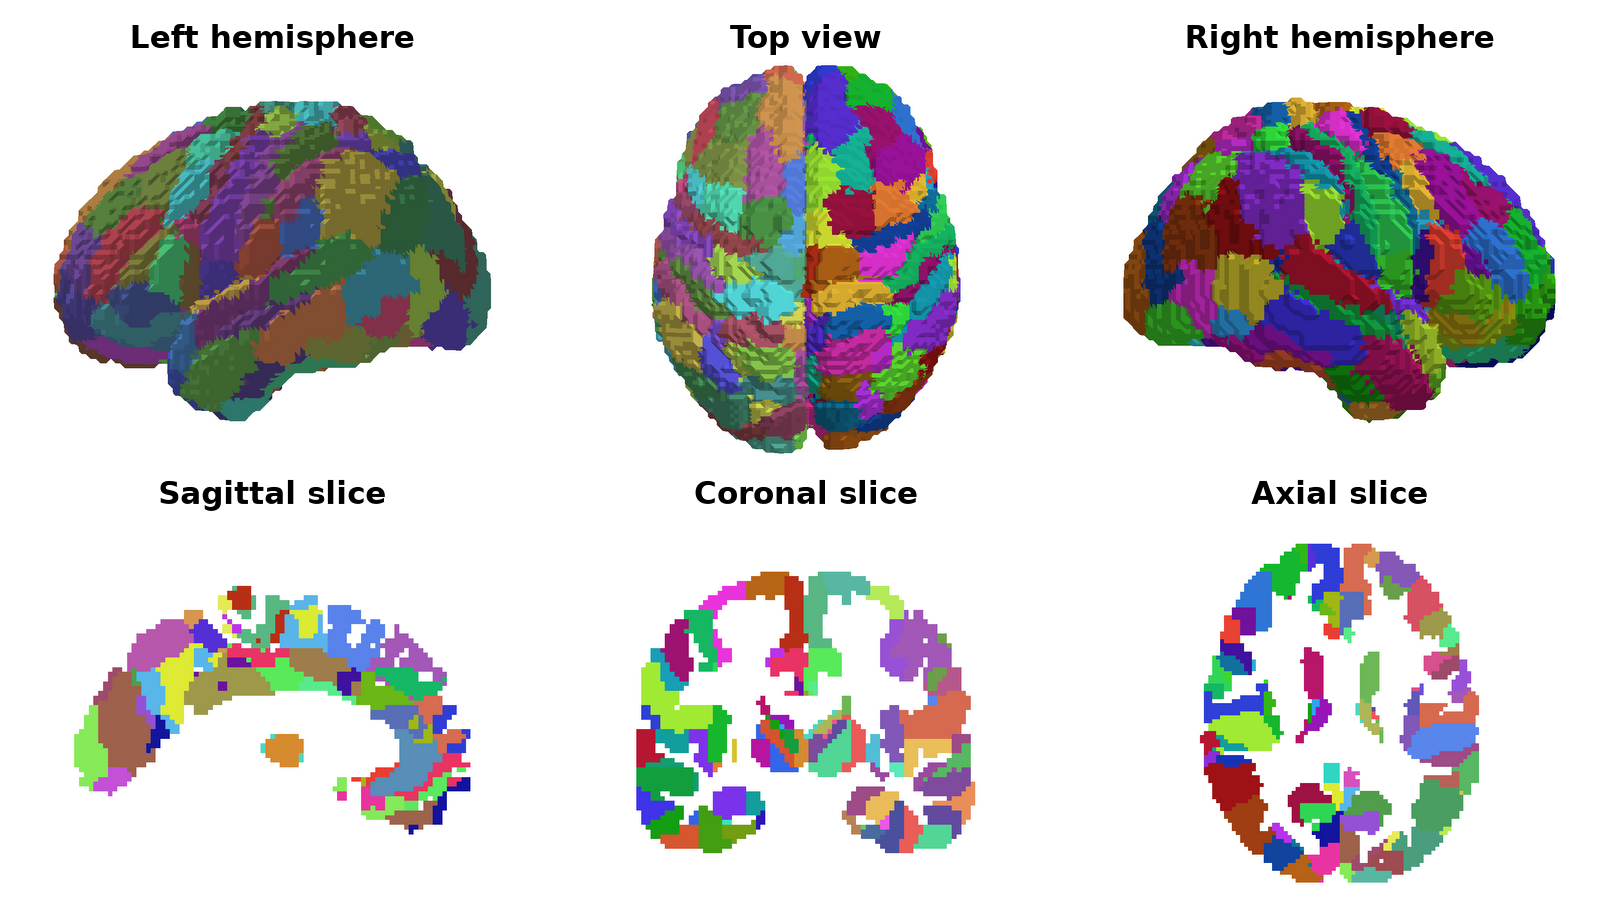
\includegraphics[width=\linewidth]{figures/atlas_overview.png}
    \column{0.34\textwidth}
      \footnotesize
      \begin{itemize}
        \item An \textbf{atlas} divides the brain into named regions so scans can be compared
              region by region.
        \item \textbf{Brainnetome atlas:} 246 regions, 123 per hemisphere \cite{r3}.
              Each colour is one region.
        \item Every scan is warped to a common template (MNI space), so region $k$ is the same
              place in every person.
        \item A region's signal is the average of its voxels: \textbf{246 time series per scan}.
      \end{itemize}
  \end{columns}
\end{frame}

% 11. Brainnetome-246 parcellation as the feature-extraction space (compact and visual)
\begin{frame}{Brainnetome 246-ROI Parcellation for Feature Extraction}
  \centering
  {\small\itshape\color{UniversityBlue} Fine-grained, whole-brain representation for systematic regional
   and inter-regional feature extraction\par}
  \vspace{0.05cm}
  \begin{columns}[T,onlytextwidth]
    \column{0.30\textwidth}
      \centering
      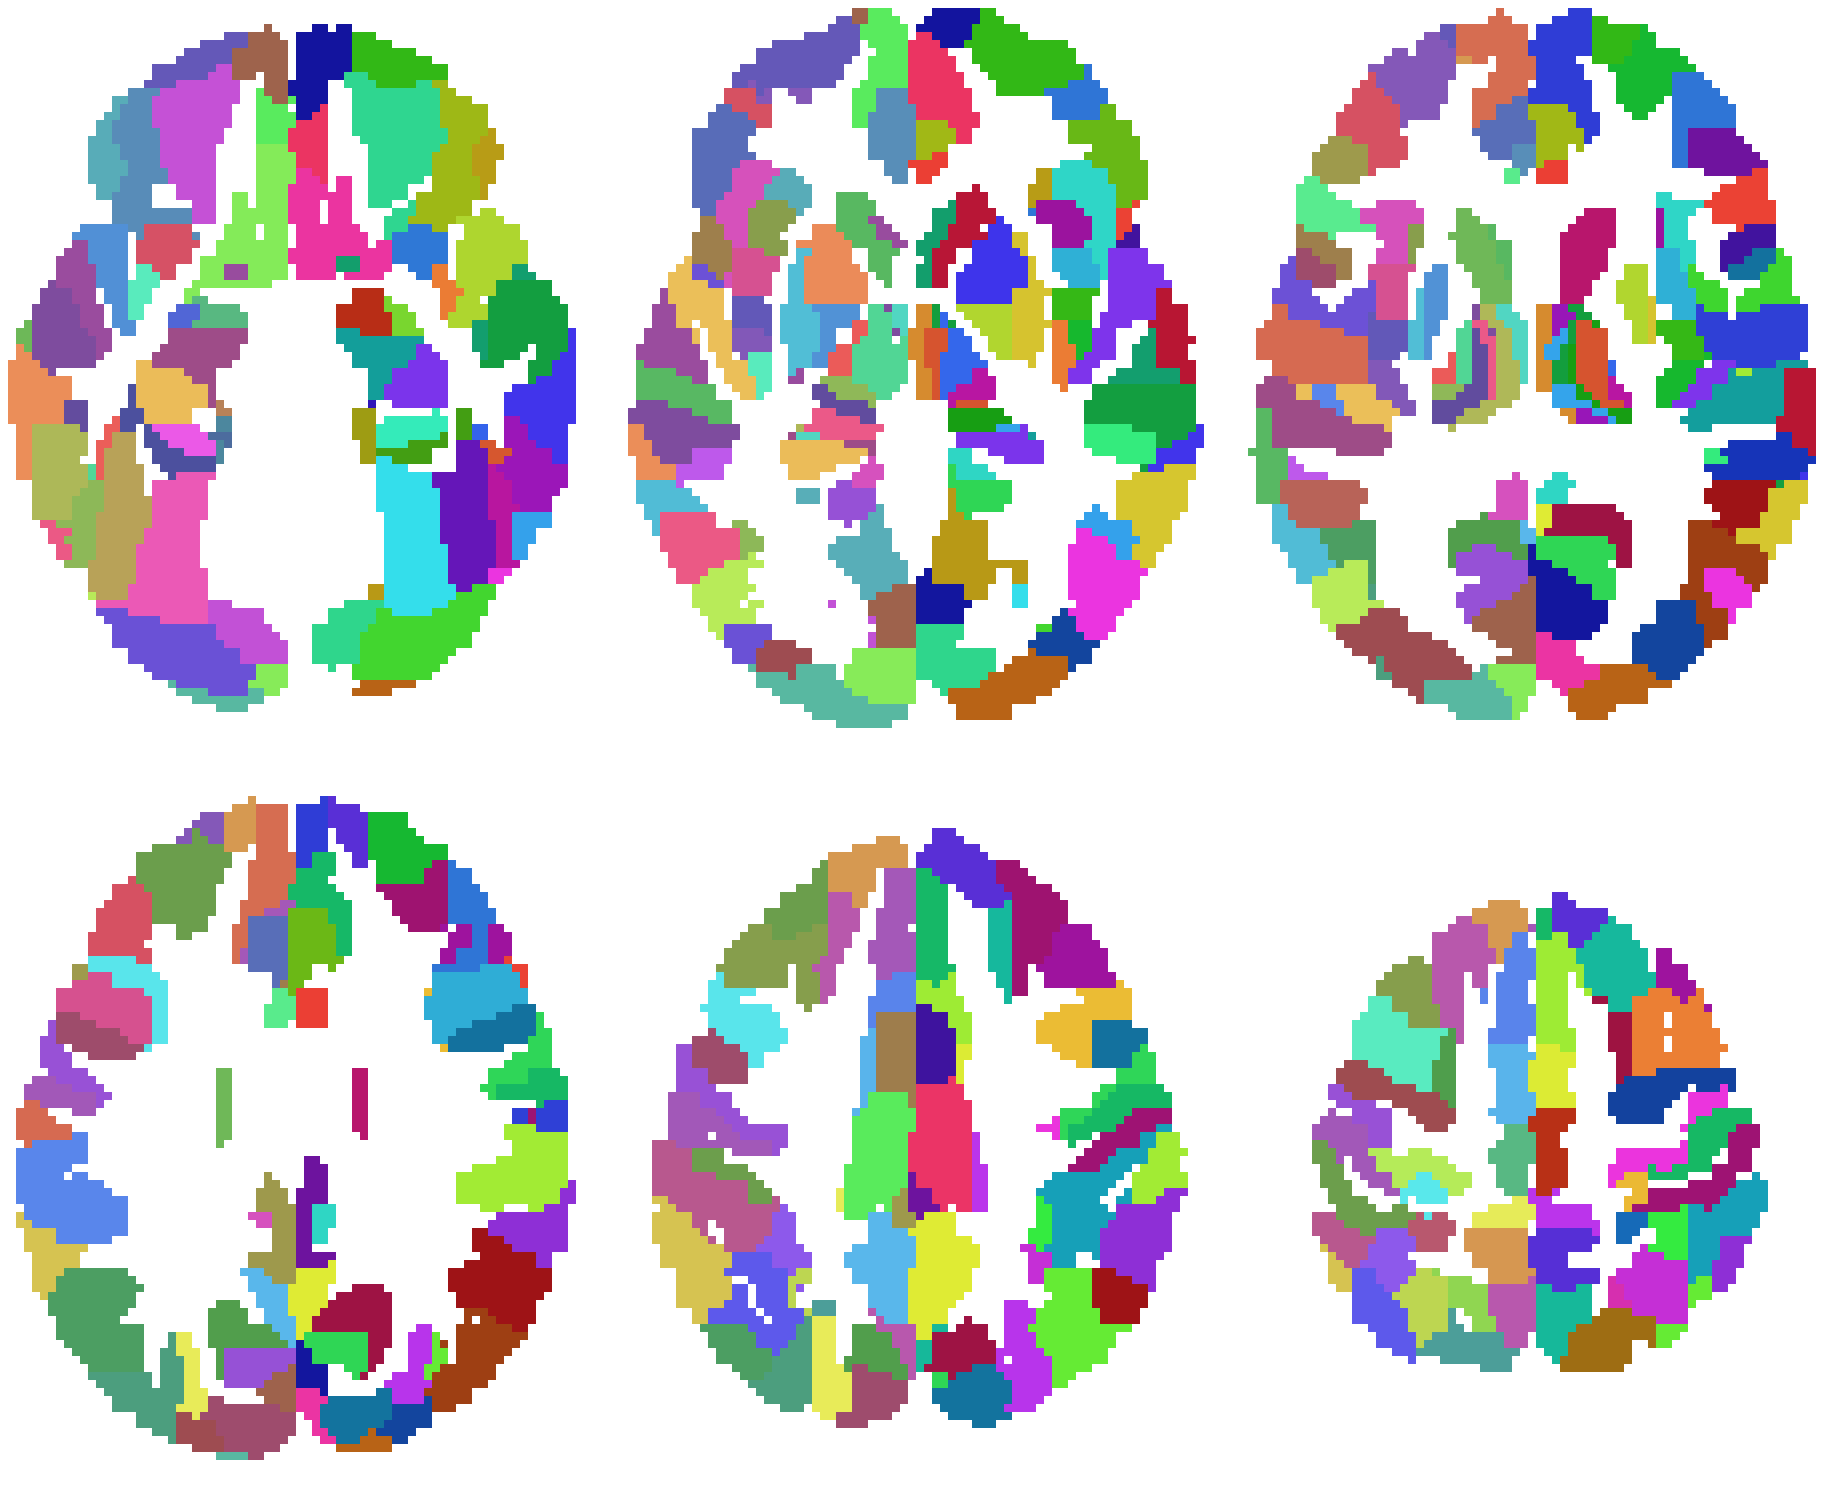
\includegraphics[width=\linewidth]{figures/atlas_axial_panel.png}\\[1pt]
      {\scriptsize Axial slices, $z=-16$ to $+56$\,mm.\\ Each colour is one ROI.}
    \column{0.69\textwidth}
      \footnotesize\raggedright
      \begin{itemize}\setlength{\itemsep}{2pt}
        \item \textbf{Fine-grained whole-brain coverage.} 246 anatomically defined ROIs covering
              cortical and subcortical regions.
        \item \textbf{Complete extraction space.} 246/246 ROIs present across all 165 acquisitions;
              no empty or zero-variance ROIs.
        \item \textbf{Systematic feature extraction.} Each ROI provides regional biomarkers
              (ALFF, ReHo, DC) and participates in the $246\times246$ FC matrix.
        \item \textbf{No premature feature selection.} All ROIs are retained to preserve spatial
              information; predictive importance will be learned by the downstream model.
      \end{itemize}
  \end{columns}
  \vspace{0.12cm}
  
\begin{tikzpicture}[kpi/.style={rounded corners=3pt,fill=UniversityBlue,text=white,align=center,
        text width=3.3cm,minimum width=3.45cm,minimum height=0.9cm,inner sep=2pt}]
    \node[kpi] at (1.725,0)  {{\Large\bfseries 246}\\[-3pt]{\scriptsize ROIs}};
    \node[kpi] at (5.375,0)  {{\Large\bfseries 165}\\[-3pt]{\scriptsize acquisitions}};
    \node[kpi] at (9.025,0)  {{\Large\bfseries 135 $\times$ 246}\\[-3pt]{\scriptsize ROI time series per scan}};
    \node[kpi] at (12.675,0) {{\Large\bfseries 246 $\times$ 246}\\[-3pt]{\scriptsize FC matrix per scan}};
  \end{tikzpicture}\\[0.06cm]
  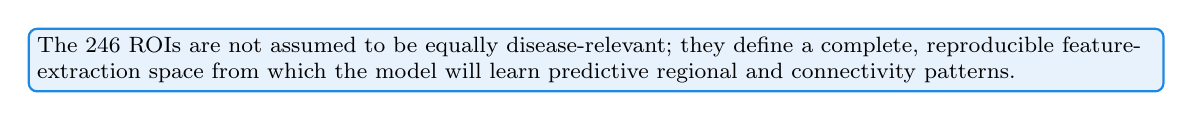
\begin{tikzpicture}
    \node[draw=AccentBlue,fill=LightBlue,rounded corners=3pt,line width=0.8pt,text width=14.2cm,
          inner sep=3pt,align=left,font=\footnotesize]
      {The 246 ROIs are not assumed to be equally disease-relevant; they define a complete,
       reproducible feature-extraction space from which the model will learn predictive regional
       and connectivity patterns.};
  \end{tikzpicture}
\end{frame}

% 12. What is new
\begin{frame}{What Is New in Our Approach}
  \small
  \begin{tabularx}{\textwidth}{>{\bfseries}p{0.8cm}>{\raggedright\arraybackslash}p{5.0cm}>{\raggedright\arraybackslash}X}
    \toprule
    & \textbf{Gap in existing work} & \textbf{What we propose (design)} \\
    \midrule
    G1 & Each biomarker is analysed on its own & \textbf{Meta-learning:} each biomarker is a task; learn a shared, biomarker-invariant representation \\[3pt]
    G2 & Clinical context is left out & \textbf{Fusion:} join covariates to the imaging representation, $H=[Z'\,\|\,C]$ \\[3pt]
    G3 & Progression treated as unordered classes & \textbf{Ordinal model} over six ordered stages \\[3pt]
    G4 & Overconfident single labels & \textbf{Bayesian output:} probability per stage with uncertainty \\
    \bottomrule
  \end{tabularx}
  \vspace{0.25cm}

  \begin{alertblock}{Honest scope}
    \footnotesize All four are \textbf{design only}: nothing is trained. Of three 2026 papers checked,
    at least one partly addresses each of G2--G4 and none addresses G1 (report \S1.3).
  \end{alertblock}
\end{frame}

% =====================================================================
% PART B. REVIEW II CONTENT
% =====================================================================

% 13. System Modules
\begin{frame}{System Modules}
  \small
  \begin{tabularx}{\textwidth}{>{\raggedright\arraybackslash}p{4.3cm}>{\centering\arraybackslash}p{1.9cm}X}
    \toprule
    \textbf{Module (Review I names)} & \textbf{Status} & \textbf{At Review II} \\
    \midrule
    1 Data/Input Management & \done & Imaging audited; clinical table cleaned (covariates for 107 of 127 subjects) \\
    2 Preprocessing Pipeline & \done & 165 of 173 scans; 8 rejected (TR 6.02\,s) \\
    3 Feature Extraction (Brainnetome 246) & \done & ALFF, ReHo, DC, FC for 165/165; normalised \\
    4 Proposed Deep Learning Model & \notst & Transformer, meta-learning, fusion: design only \\
    5 Core Output Classifier & \notst & Bayesian ordinal head: design only \\
    6 Decision Support Dashboard & \notst & No interface built \\
    \bottomrule
  \end{tabularx}
\end{frame}

% 14. Methodology / Workflow
\begin{frame}{Methodology / Workflow}
  \centering
  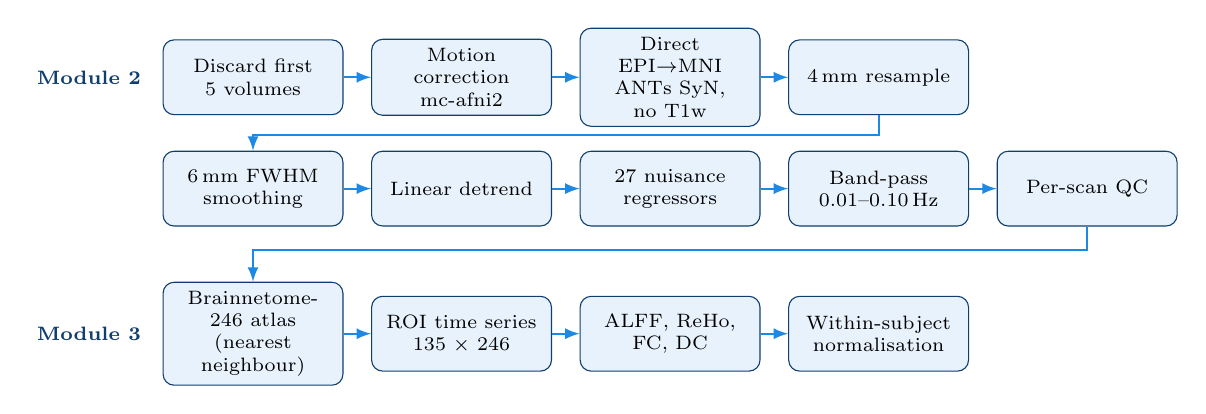
\begin{tikzpicture}[>=latex,
      st/.style={draw=UniversityBlue,fill=LightBlue,rounded corners,
                 text width=2.05cm,minimum height=0.95cm,align=center,font=\scriptsize,
                 execute at begin node={\hyphenpenalty=10000}},
      ar/.style={->,thick,draw=AccentBlue}]
    % Module 2 chain, two rows
    \node[st] (a1) {Discard first 5 volumes};
    \node[st,right=0.35cm of a1] (a3) {Motion correction\\ mc-afni2};
    \node[st,right=0.35cm of a3] (a4) {Direct EPI$\rightarrow$MNI\\ ANTs SyN, no T1w};
    \node[st,right=0.35cm of a4] (a5) {4\,mm resample};
    \node[st,below=0.45cm of a1] (b1) {6\,mm FWHM smoothing};
    \node[st,right=0.35cm of b1] (b2) {Linear detrend};
    \node[st,right=0.35cm of b2] (b3) {27 nuisance regressors};
    \node[st,right=0.35cm of b3] (b4) {Band-pass 0.01--0.10\,Hz};
    \node[st,right=0.35cm of b4] (b5) {Per-scan QC};
    % Module 3 chain
    \node[st,below=0.7cm of b1] (c1) {Brainnetome-246 atlas (nearest neighbour)};
    \node[st,right=0.35cm of c1] (c2) {ROI time series\\ $135\times246$};
    \node[st,right=0.35cm of c2] (c3) {ALFF, ReHo, FC, DC};
    \node[st,right=0.35cm of c3] (c4) {Within-subject normalisation};
    \foreach \x/\y in {a1/a3,a3/a4,a4/a5,b1/b2,b2/b3,b3/b4,b4/b5,c1/c2,c2/c3,c3/c4}
      \draw[ar] (\x) -- (\y);
    \draw[ar] (a5.south) -- ++(0,-0.25) -| (b1.north);
    \draw[ar] (b5.south) -- ++(0,-0.3) -| (c1.north);
    \node[font=\scriptsize\bfseries,text=UniversityBlue,anchor=east] at ([xshift=-0.15cm]a1.west) {Module 2};
    \node[font=\scriptsize\bfseries,text=UniversityBlue,anchor=east] at ([xshift=-0.15cm]c1.west) {Module 3};
  \end{tikzpicture}
  \vspace{0.3cm}

  \small Every step is checked per acquisition; a scan that fails a check is logged, never silently altered.
\end{frame}

% 15. Preprocessing explained
\begin{frame}{Preprocessing: What Each Step Does and Why}
  \footnotesize
  \begin{tabularx}{\textwidth}{>{\bfseries\raggedright\arraybackslash}p{3.6cm}>{\raggedright\arraybackslash}p{4.5cm}>{\raggedright\arraybackslash}X}
    \toprule
    Step & What it does & Why it is needed \\
    \midrule
    Discard first 5 volumes & drops the first 15\,s & the signal is still settling at the start \\[2pt]
    Motion correction & aligns every volume to the first & head movement would otherwise look like brain activity \cite{r8,r9} \\[2pt]
    Warp to MNI template & maps each brain onto a standard brain \cite{r10} & so region $k$ is the same place in every person \\[2pt]
    Resample to 4\,mm, smooth 6\,mm & coarser grid and slight blur & less noise and fewer voxels \\[2pt]
    Detrend and 27 regressors & removes slow drift and motion, white-matter and whole-brain signal & non-neural influences hide the neural signal \\[2pt]
    Band-pass 0.01--0.10\,Hz & keeps only slow fluctuations & the range where resting-state activity lives \\[2pt]
    Quality control & motion, signal-to-noise and file checks per scan & failures are logged, never silently altered \\
    \bottomrule
  \end{tabularx}
\end{frame}

% 16. Core Algorithm - implemented
\begin{frame}{Core Algorithm A: Implemented Biomarkers and Normalisation}
  \begin{columns}[T,onlytextwidth]
    \column{0.47\textwidth}
      \begin{block}{Biomarkers (per Brainnetome region)}
        \footnotesize
        \begin{itemize}
          \item \textbf{ALFF:} mean FFT amplitude, 0.01--0.10\,Hz
          \item \textbf{ReHo:} Kendall's $W$, 27-voxel neighbourhood
          \item \textbf{FC:} $246\times246$ Pearson, signed, unthresholded
          \item \textbf{DC:} $\mathrm{DC}_i=\sum_{j\neq i}\mathrm{FC}_{ij}$
        \end{itemize}
      \end{block}
    \column{0.51\textwidth}
      \begin{block}{Within-subject normalisation}
        \footnotesize
        \begin{itemize}
          \item mALFF $=\mathrm{ALFF}_i/\overline{\mathrm{ALFF}}$
          \item mReHo $=\mathrm{ReHo}_i/\overline{\mathrm{ReHo}}$
          \item $\mathrm{DC}_z=(\mathrm{DC}_i-\overline{\mathrm{DC}})/\sigma_{\mathrm{DC}}$
          \item FC $\rightarrow\operatorname{artanh}\bigl(\operatorname{clip}(r,\pm0.999999)\bigr)$, diagonal $=0$
        \end{itemize}
      \end{block}
  \end{columns}
  \vspace{0.2cm}
  \begin{itemize}
    \item Every statistic comes from \textbf{one acquisition's own 246 values}.
    \item No cross-subject statistic and no label: leakage-free by construction.
    \item Verified: mean(mALFF) = mean(mReHo) = 1.000000; std(DC$_z$) = 1.000000 (165/165).
    \item 0 off-diagonal entries needed clipping; Fisher-$z$ diagonal exactly 0.
  \end{itemize}
\end{frame}

% 17. Implementation Status
\begin{frame}{Implementation Status}
  \centering
  \resizebox{0.8\textwidth}{!}{%
  \begin{ganttchart}[
      x unit=1.05cm, y unit chart=0.5cm, y unit title=0.5cm,
      title height=1, title label font=\small, bar label font=\small,
      milestone label font=\small, vgrid={*{1}{draw=none},dotted},
      hgrid, bar height=0.55,
      bar/.append style={fill=green!35!black!45},
      bar incomplete/.append style={fill=gray!22},
      progress label text={},
      milestone/.append style={fill=red!60},
      vrule/.style={very thick, red!70!black}]{1}{8}
    \gantttitle{Aug}{1}\gantttitle{Sep}{1}\gantttitle{Oct}{1}\gantttitle{Nov}{1}\gantttitle{Dec}{1}\gantttitle{Jan}{1}\gantttitle{Feb}{1}\gantttitle{Mar}{1}\\
    \ganttbar[progress=100]{Literature, problem \& design}{1}{1}\\
    \ganttbar[progress=100]{M2: Preprocessing \& validation}{2}{2}\\
    \ganttbar[progress=100]{M3: Feature extraction (BN-246)}{3}{3}\\
    \ganttbar[progress=0]{M4 \& M5: Transformer, classifier}{5}{6}\\
    \ganttbar[progress=0]{Testing and evaluation}{7}{7}\\
    \ganttbar[progress=0]{Documentation}{7}{8}\\
    \ganttmilestone{Final submission}{8}
    \ganttvrule{Review II (Phase 1 final)}{3}
  \end{ganttchart}}
  \vspace{0.15cm}

  \begin{alertblock}{One milestone ahead of the Review I plan}
    Module 2 was planned for Review II and Module 3 for Review III.
    \textbf{Both are complete at Review II}, the final review of Phase 1.
  \end{alertblock}
  {\footnotesize Applies to the \textbf{data foundation only} (Modules 1--3); Modules 4--6 are not started.
  Module 2 completed in September; Module 3 in October (normalised biomarkers 5 Oct).}
\end{frame}

% 18. Results: data-stage only
\begin{frame}{Results: Data Foundation Verification}
  \begin{alertblock}{}
    \small These are \textbf{data-stage} results. \textbf{No model performance exists.}
  \end{alertblock}
  \vspace{0.1cm}
  \begin{columns}[T,onlytextwidth]
    \column{0.52\textwidth}
      \small
      \begin{tabular}{lr}
        \toprule
        \textbf{Check (165 acquisitions)} & \textbf{Result} \\
        \midrule
        246/246 regions covered & 165/165 \\
        ROI series $(135,246)$ & 165/165 \\
        NaN / Inf / zero-variance & 0 / 0 / 0 \\
        Pilot reproduction & bit-identical \\
        DC recomputed from FC, max diff. & \alert{0.000e+00} \\
        Consistency checks passed & 165/165 \\
        \bottomrule
      \end{tabular}
    \column{0.46\textwidth}
      \small
      \begin{itemize}
        \item \alert{127 subjects, not 165 scans}: 96 have one scan, 25 two, 5 three, 1 four.
        \item Smallest class: MCI, 32 scans but only \textbf{14 subjects}.
        \item QC medians ($n=164$, one artefact scan excluded): tSNR 127.95, SNR 13.12, FD 0.317\,mm.
      \end{itemize}
  \end{columns}
\end{frame}

% 19. How to read the heatmaps
\begin{frame}{How to Read the Stage Heatmaps}
  \begin{columns}[T,onlytextwidth]
    \column{0.42\textwidth}
      \centering
      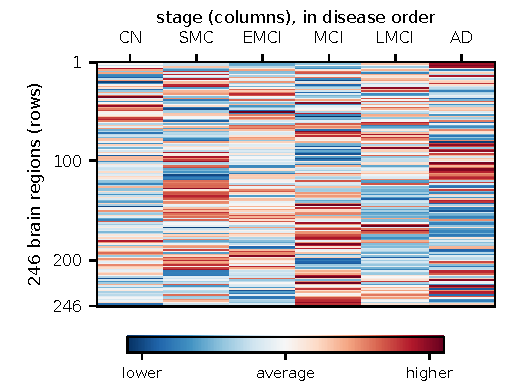
\includegraphics[width=\linewidth]{figures/malff_annotated.pdf}\par
      {\scriptsize mALFF, 127 subjects (real data).}
    \column{0.56\textwidth}
      \footnotesize
      \begin{itemize}
        \item Each \textbf{row} is a brain region (246), each \textbf{column} a stage. A cell is the
              group average for that stage.
        \item \textbf{Colour} is relative to the region's own average over the six stages
              (row-wise $z$-score): absolute levels are removed on purpose.
        \item Disease-driven change would appear as a row shifting \textbf{steadily} from one colour
              to the other, left to right.
        \item \textbf{By chance}, an unrelated region is steadily ordered with probability
              $2/6!\approx0.28\%$: about \textbf{0.7 of 246 regions}. We found 1, 0 and 1.
      \end{itemize}
      \vspace{0.05cm}
      \centering
      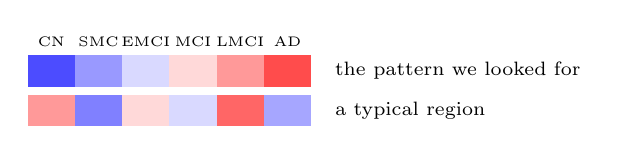
\begin{tikzpicture}[x=0.6cm,y=0.5cm]
        \foreach \i/\s in {0/CN,1/SMC,2/EMCI,3/MCI,4/LMCI,5/AD} \node[font=\tiny] at (\i+0.5,1.15) {\s};
        \foreach \i/\c in {0/blue!70,1/blue!40,2/blue!15,3/red!15,4/red!40,5/red!70}
          \fill[\c] (\i,0) rectangle (\i+1,0.8);
        \foreach \i/\c in {0/red!40,1/blue!50,2/red!15,3/blue!15,4/red!60,5/blue!35}
          \fill[\c] (\i,-1.0) rectangle (\i+1,-0.2);
        \node[anchor=west,font=\scriptsize] at (6.3,0.4) {the pattern we looked for};
        \node[anchor=west,font=\scriptsize] at (6.3,-0.6) {a typical region};
      \end{tikzpicture}\par
      {\tiny schematic, not data}
  \end{columns}
\end{frame}

% 20. Results: finding 1
\begin{frame}{Finding 1: FC Strength Equals DC/245}
  \begin{columns}[T,onlytextwidth]
    \column{0.52\textwidth}
      \begin{block}{Review I fourth column was redundant}
        \footnotesize
        \begin{equation*}
          \mathrm{FCS}_i=\frac{1}{245}\sum_{j\neq i}\mathrm{FC}_{ij}=\frac{\mathrm{DC}_i}{245}
        \end{equation*}
        \vspace{-6pt}
      \end{block}
      \small
      \begin{itemize}
        \item Max difference \textbf{6.939e-18}; Pearson $r=1.000000000000$.
        \item \textbf{All four biomarkers are kept.}
        \item ALFF, ReHo, DC: $246\times3$ regional matrix.
        \item FC: full $246\times246$ Fisher-$z$ matrix.
        \item A design correction found by auditing our own features.
      \end{itemize}
    \column{0.46\textwidth}
      \centering
      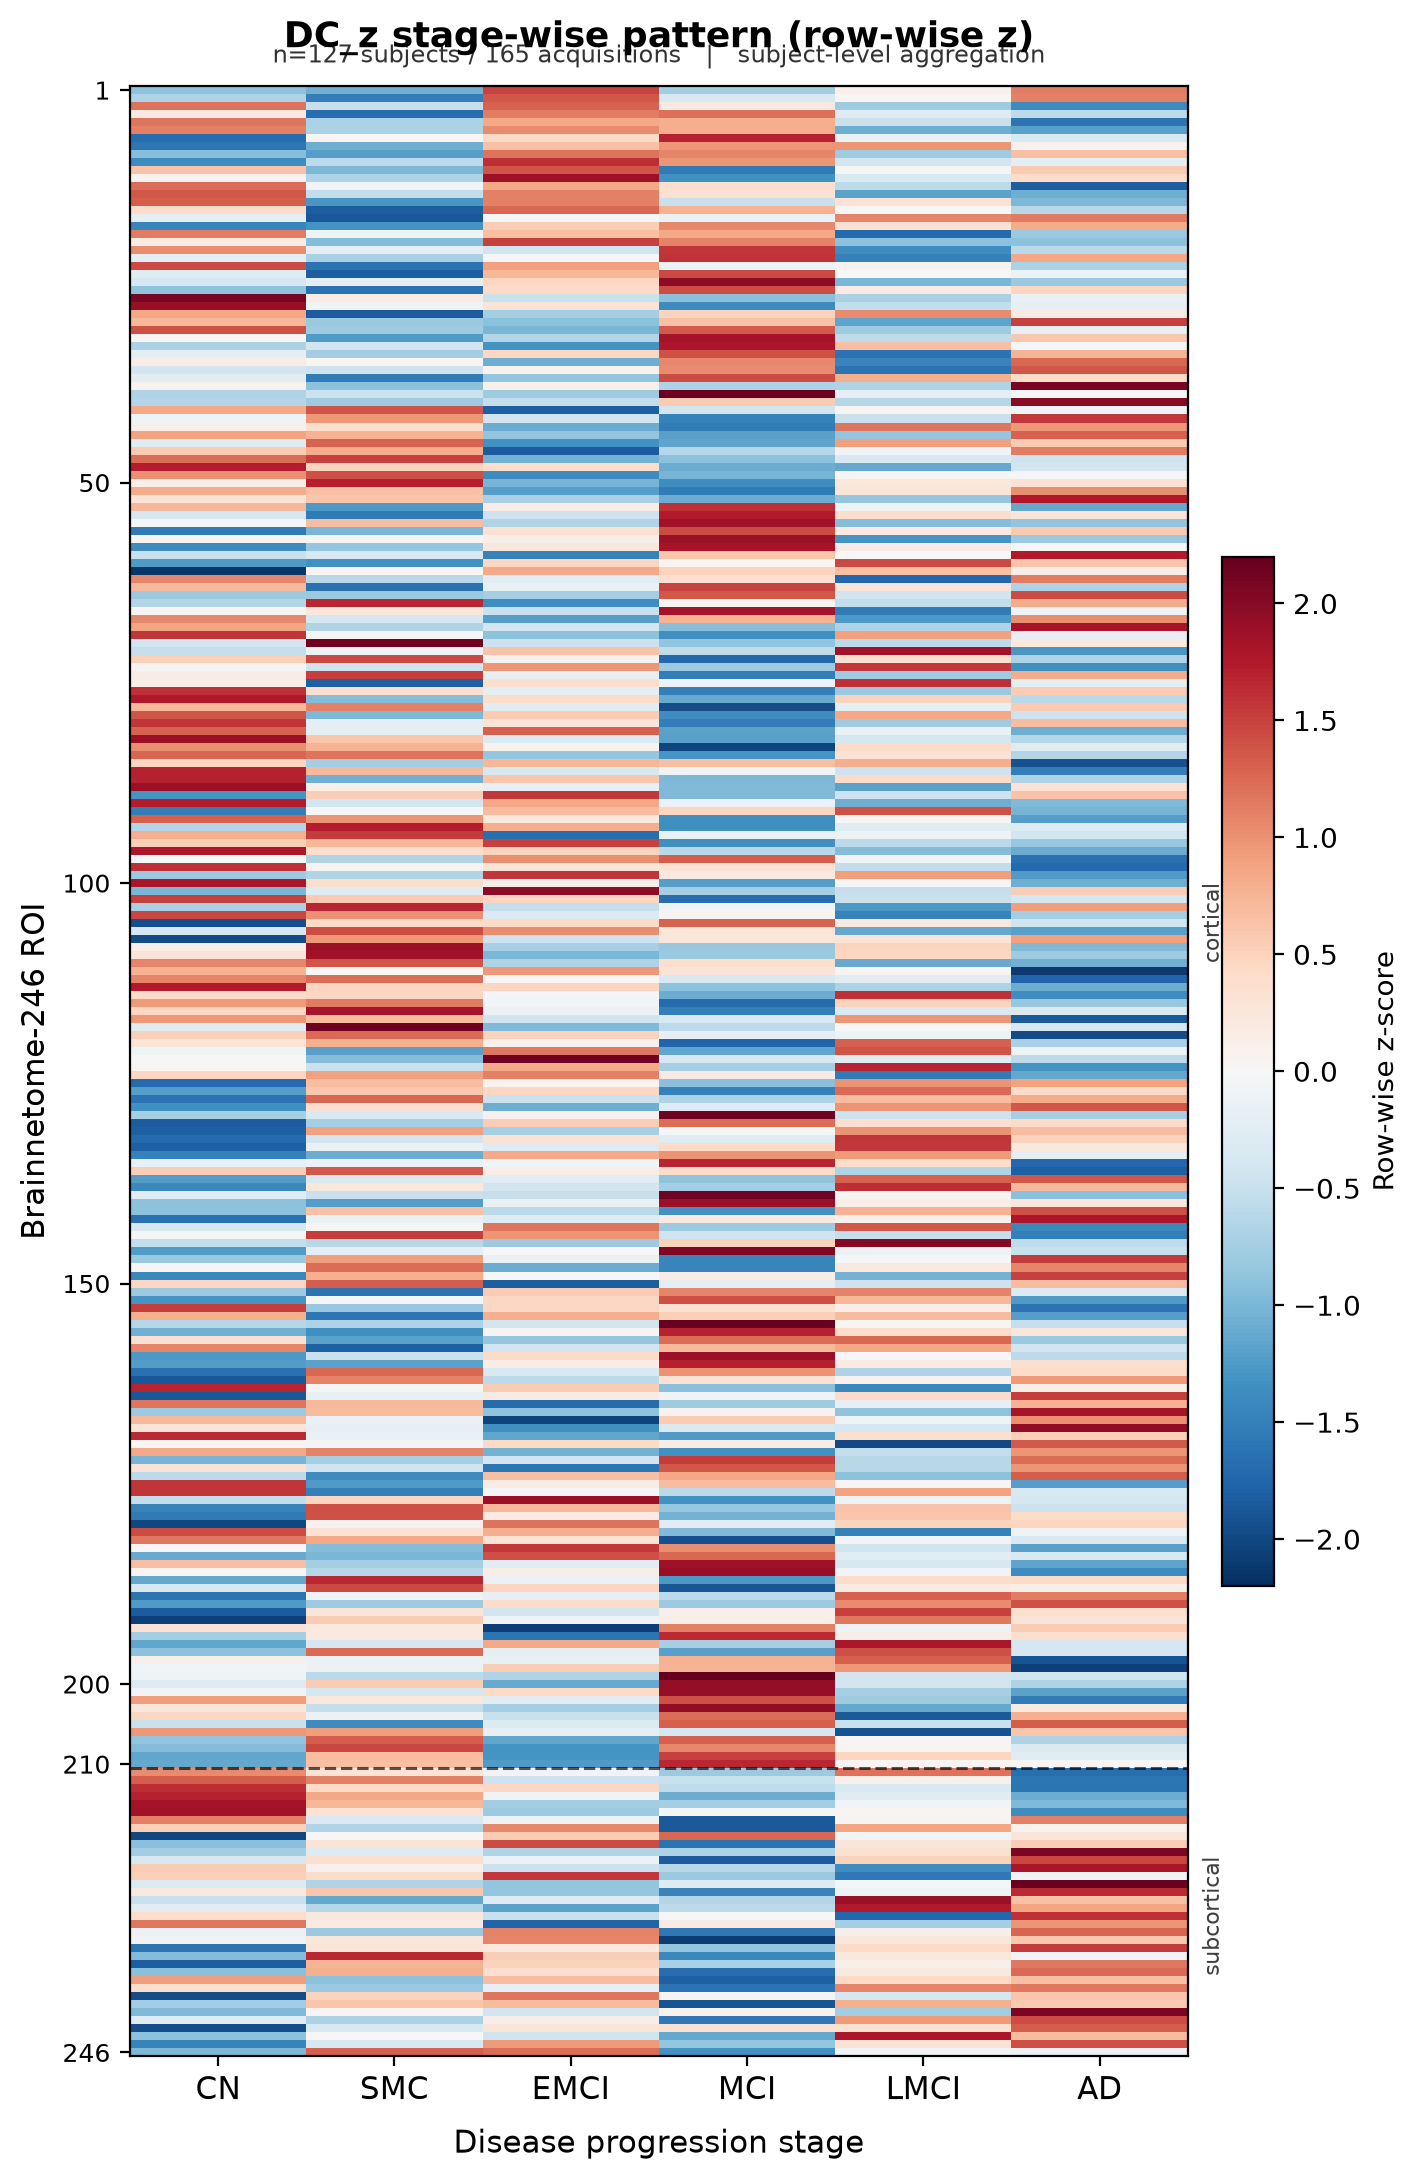
\includegraphics[height=4.0cm]{figures/DC_z_rowz.png}\,
      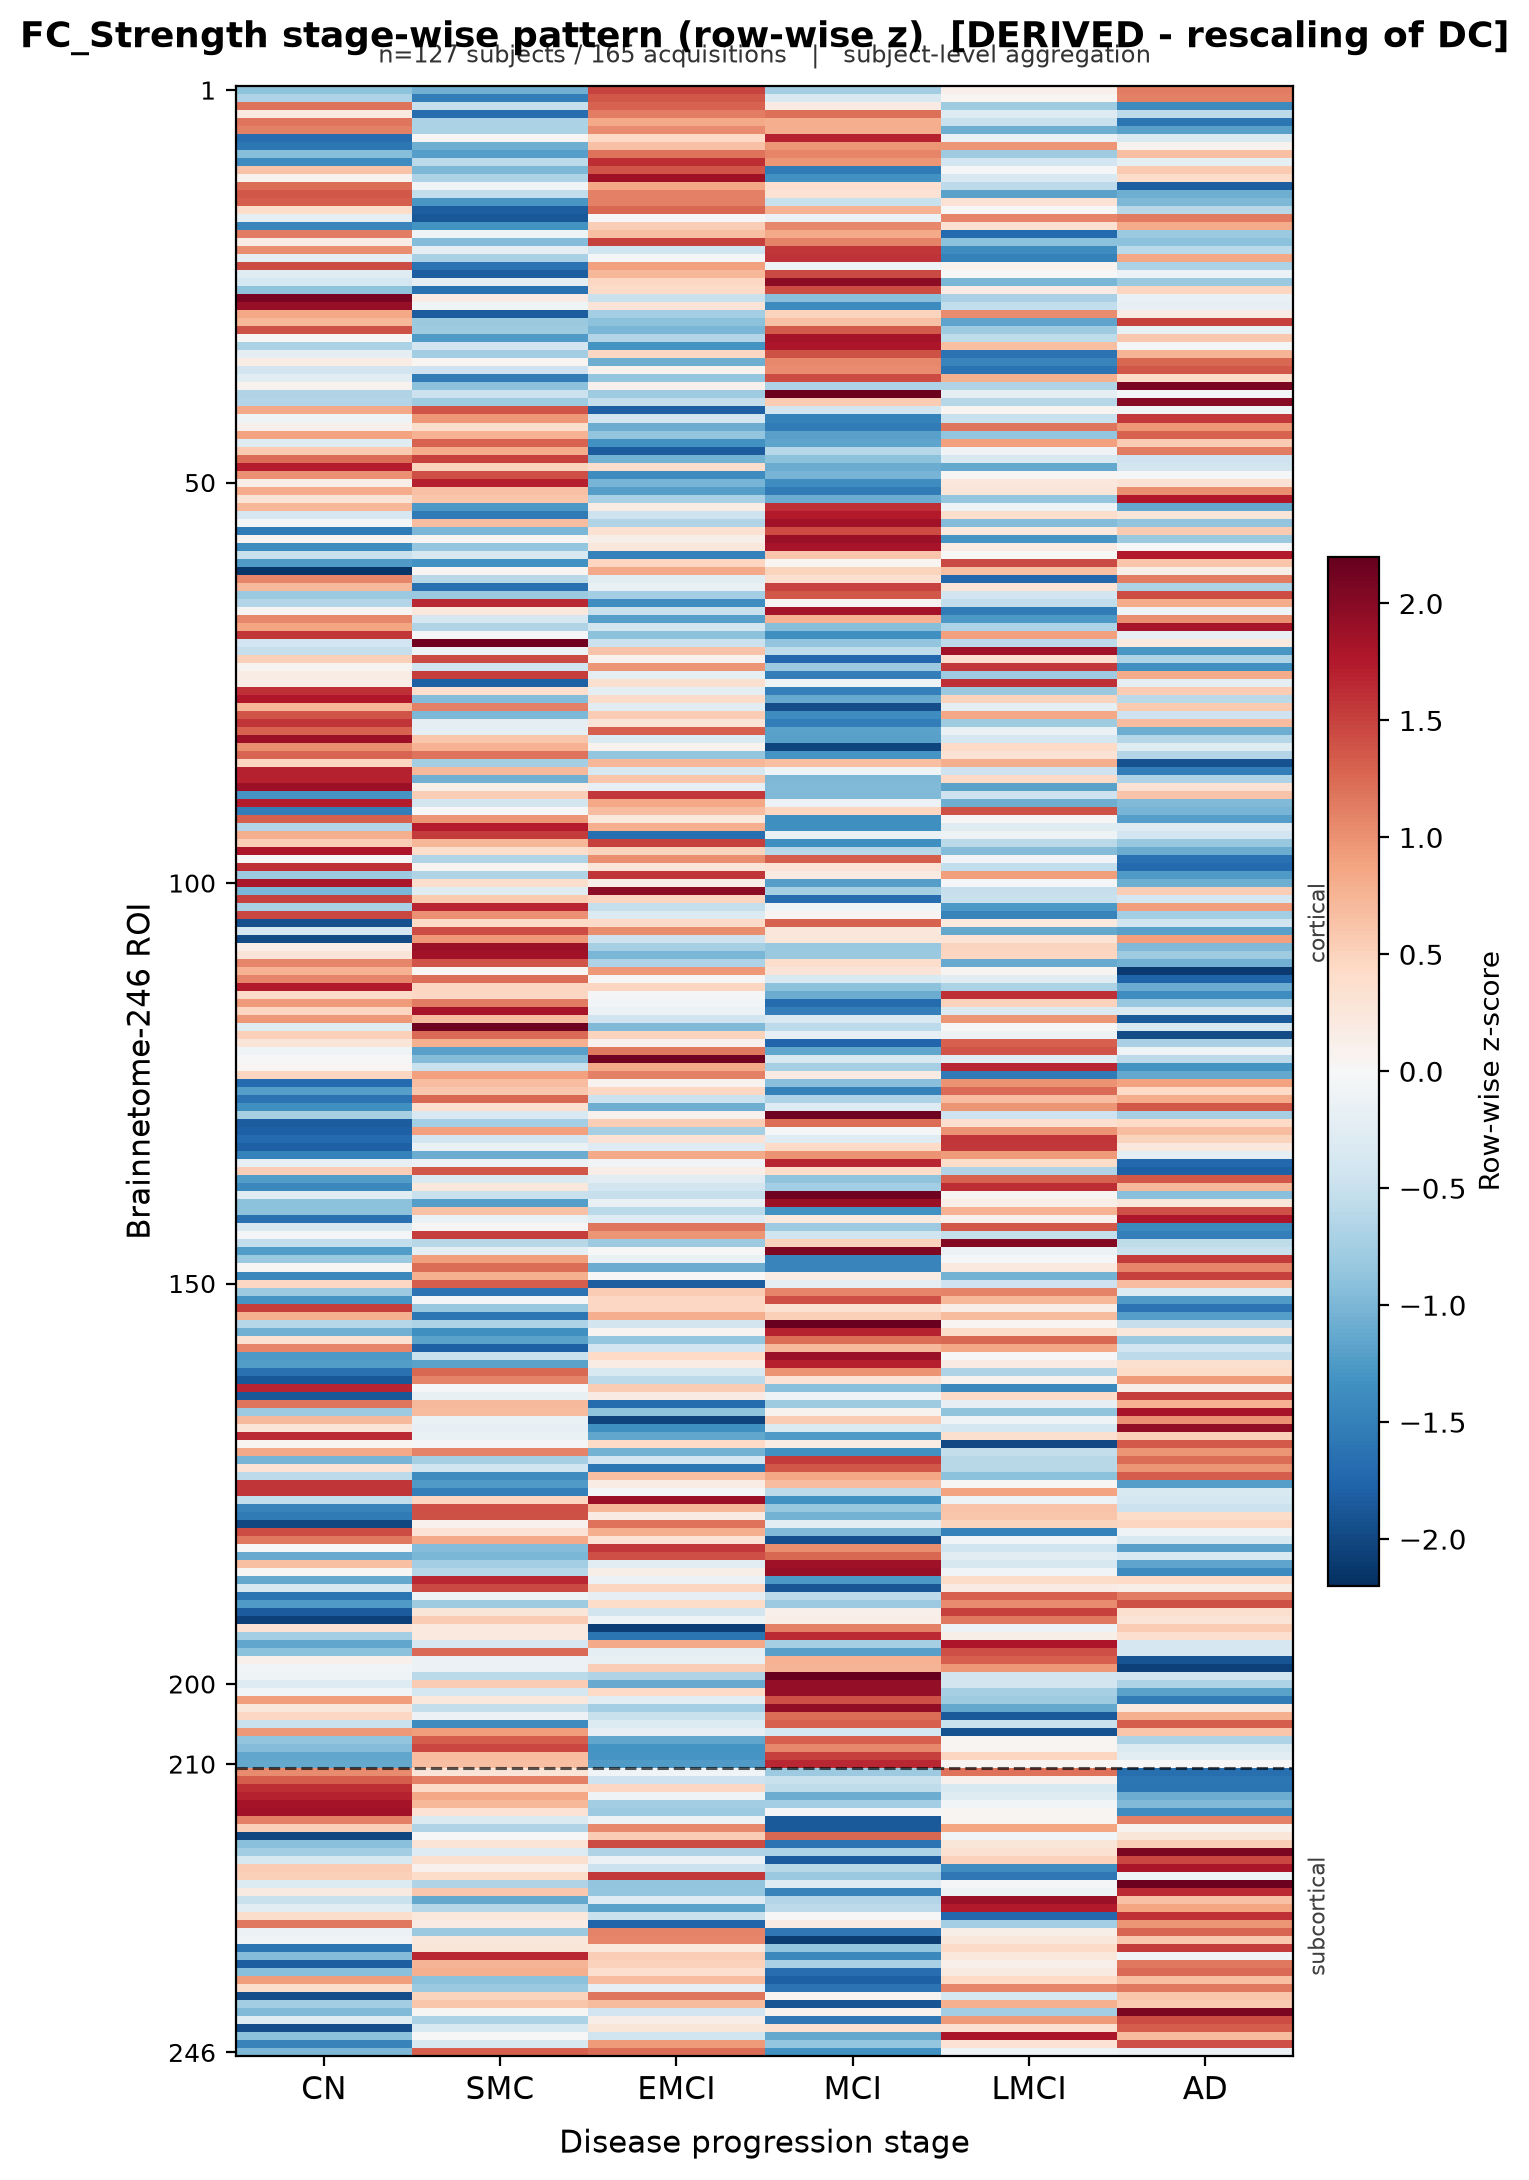
\includegraphics[height=4.0cm]{figures/FC_Strength_rowz.png}

      {\scriptsize DC$_z$ (left) and FC\_Strength (right): identical panels, as expected.
      Descriptive and exploratory only.}
  \end{columns}
\end{frame}

% 21. Results: finding 2
\begin{frame}{Finding 2: No Univariate Progression Signal}
  \begin{columns}[T,onlytextwidth]
    \column{0.50\textwidth}
      \centering
      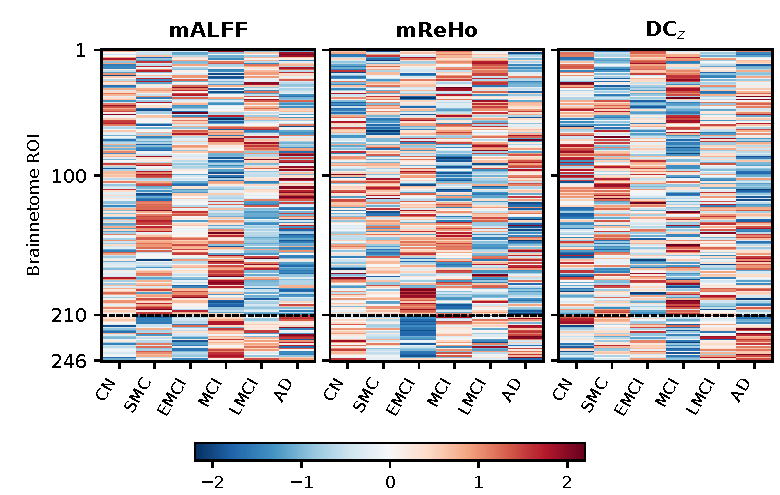
\includegraphics[width=\linewidth]{figures/stage_rowz_panel_slide.pdf}

      {\scriptsize Stage-wise row-$z$ patterns, 127 subjects (CN$\to$AD).
      Descriptive and exploratory; no statistical test.}
    \column{0.48\textwidth}
      \footnotesize
      \begin{tabular}{lcc}
        \toprule
        & \textbf{Monotonic CN$\to$AD} & \textbf{By chance} \\
        \midrule
        mALFF & 1 / 246 & $\approx0.7$ \\
        mReHo & 0 / 246 & $\approx0.7$ \\
        DC$_z$ & 1 / 246 & $\approx0.7$ \\
        \bottomrule
      \end{tabular}
      \vspace{0.2cm}
      \small
      \begin{itemize}
        \item No more than chance; stage variation is 4--5$\times$ below anatomy.
        \item Informative, not a failure.
        \item Group means discard the whole connectivity structure.
        \item \textbf{Motivates the multivariate model.}
      \end{itemize}
  \end{columns}
\end{frame}

% 22. Results: finding 3
\begin{frame}{Finding 3: The Biomarkers Are Not Redundant}
  \centering
  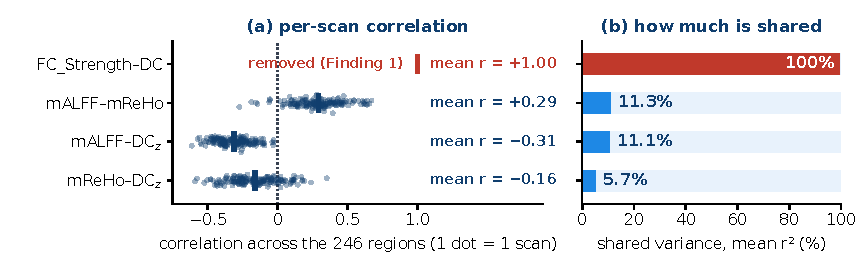
\includegraphics[width=\textwidth]{figures/findings_complementarity.pdf}\\[2pt]
  \footnotesize\raggedright
  FC strength equals DC/245 exactly (Finding 1) and was removed. The three kept biomarkers share only
  \textbf{6--11\,\%} of their variance across the 246 regions (\textbf{89--94\,\% non-redundant}, all 165 scans),
  and mALFF and DC$_z$ are negatively related in every scan.\par
  \vspace{0.15cm}
  \begin{block}{}
    \footnotesize Gap G1 uses each biomarker as a separate task. That only makes sense if they carry different
    information, and they overlap little. Whether it improves staging is untested (Phase 2).
  \end{block}
\end{frame}

% 23. Results: finding 4
\begin{frame}{Finding 4: The Features Are Reproducible and Plausible}
  \centering
  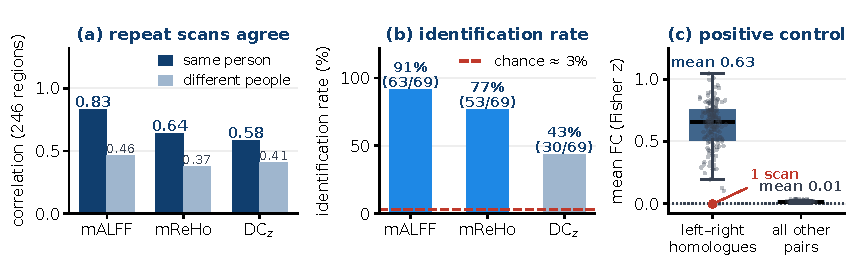
\includegraphics[width=\textwidth]{figures/findings_reliability.pdf}\\[2pt]
  \footnotesize\raggedright
  \textbf{31 people} have repeat scans (69 scans; 45 of 46 pairs are from different sessions). For mALFF, a scan's
  closest match is the same person's other scan in \textbf{63 of 69} cases (chance $\approx$\,3\,\%), and left--right
  homologous regions are strongly connected in \textbf{164 of 165} scans (one EMCI scan lacks this and needs checking).\par
  \vspace{0.15cm}
  \begin{block}{}
    \footnotesize Data checks, not a disease classifier: no stage label is used. A person's repeat scans usually share a
    site and scanner, so part of the reproducibility may be scanner-related.
  \end{block}
\end{frame}

% 24. Team Responsibilities
\begin{frame}{Team Responsibilities}
  \small
  \begin{tabularx}{\textwidth}{>{\bfseries\raggedright\arraybackslash}p{3.3cm}>{\raggedright\arraybackslash}p{5.6cm}>{\raggedright\arraybackslash}X}
    \toprule
    Team member & Responsibility & Status at Review II \\
    \midrule
    Harishkanna R & Preprocessing (Module 2); transformer model (Module 4) & Preprocessing: \done\newline Transformer: \notst \\
    Dhananchezhiyan M & Meta-Bayesian module (meta-learning, Bayesian classifier) and final module (dashboard) & \notst \\
    Nagindhar Sachein R L & Dataset cleaning (clinical and comorbidity tables, dataset expansion) & Clinical cleaning done and audited; dataset expansion next \\
    \bottomrule
  \end{tabularx}
  \vspace{0.3cm}

  {\footnotesize Feature extraction (Module 3) was completed by the team and is verified.}
\end{frame}

% 25. References
\begin{frame}{References}
  \setbeamertemplate{bibliography item}[text]
  \fontsize{6}{7}\selectfont
  \begin{multicols}{2}
  \begin{thebibliography}{99}
    \bibitem{r1} C. R. Jack Jr. \emph{et al.}, ``ADNI: MRI methods,'' \emph{J. Magn. Reson. Imaging}, 27(4), 2008.
    \bibitem{r2} R. C. Petersen \emph{et al.}, ``ADNI: clinical characterization,'' \emph{Neurology}, 74(3), 2010.
    \bibitem{r3} L. Fan \emph{et al.}, ``The Human Brainnetome Atlas,'' \emph{Cerebral Cortex}, 26(8), 2016.
    \bibitem{r4} Y. Zang \emph{et al.}, ``Regional homogeneity approach to fMRI data analysis,'' \emph{NeuroImage}, 22(1), 2004.
    \bibitem{r5} Y.-F. Zang \emph{et al.}, ``Altered baseline brain activity in children with ADHD,'' \emph{Brain Dev.}, 29(2), 2007.
    \bibitem{r6} Q.-H. Zou \emph{et al.}, ``An improved approach to detection of ALFF: fractional ALFF,'' \emph{J. Neurosci. Methods}, 172(1), 2008.
    \bibitem{r7} X.-N. Zuo \emph{et al.}, ``Network centrality in the human functional connectome,'' \emph{Cereb. Cortex}, 22(8), 2012.
    \bibitem{r8} J. D. Power \emph{et al.}, ``Spurious but systematic correlations in functional connectivity MRI,'' \emph{NeuroImage}, 59(3), 2012.
    \bibitem{r9} K. J. Friston \emph{et al.}, ``Movement-related effects in fMRI time-series,'' \emph{Magn. Reson. Med.}, 35(3), 1996.
    \bibitem{r10} B. B. Avants \emph{et al.}, ``Symmetric diffeomorphic image registration with cross-correlation,'' \emph{Med. Image Anal.}, 12(1), 2008.
    \bibitem{r11} B. Fischl, ``FreeSurfer,'' \emph{NeuroImage}, 62(2), 2012.
    \bibitem{r12} R. W. Cox, ``AFNI: software for analysis of functional MR neuroimages,'' \emph{Comput. Biomed. Res.}, 29(3), 1996.
    \bibitem{r13} A. Vaswani \emph{et al.}, ``Attention is all you need,'' \emph{NeurIPS}, 30, 2017.
    \bibitem{r14} C. Finn, P. Abbeel, S. Levine, ``Model-agnostic meta-learning,'' \emph{ICML}, 2017.
    \bibitem{r15} Y. Gal, Z. Ghahramani, ``Dropout as a Bayesian approximation,'' \emph{ICML}, 2016.
    \bibitem{r16} P. McCullagh, ``Regression models for ordinal data,'' \emph{J. R. Stat. Soc. B}, 42(2), 1980.
    \bibitem{r17} A. Hariharan, S. N. Gowda, Anala M R, ``Uncertainty-aware longitudinal forecasting of AD progression,'' arXiv:2606.24604, 2026.
    \bibitem{r18} B.-S. Rauchmann \emph{et al.}, ``Multimodal ordinal modeling of AD severity (MRI and clinical),'' arXiv:2606.11794, 2026.
    \bibitem{r19} K. Alsalem \emph{et al.}, ``Progression-aware CNN--Transformer for multiclass AD staging,'' \emph{Diagnostics}, 16(4):593, 2026.
  \end{thebibliography}
  \end{multicols}
\end{frame}

% 26. Thank you
\begin{frame}[plain]
  \centering
  \vfill
  {\usebeamerfont{title}\color{UniversityBlue}\Huge Thank You}\par
  \vspace{0.5cm}
  {\Large Questions and Discussion}\par
  \vspace{0.8cm}
  \vfill
\end{frame}

% =====================================================================
% BACKUP SLIDES (not counted in the page numbers)
% =====================================================================
\appendix

% B1. Glossary
\begin{frame}{Backup: Glossary}
  \scriptsize
  \begin{tabularx}{\textwidth}{>{\bfseries\raggedright\arraybackslash}p{1.9cm}>{\raggedright\arraybackslash}X>{\bfseries\raggedright\arraybackslash}p{1.9cm}>{\raggedright\arraybackslash}X}
    \toprule
    Term & Meaning & Term & Meaning \\
    \midrule
    rs-fMRI & functional MRI recorded while the person rests & ALFF & amplitude of low-frequency fluctuations: size of the slow signal swings \\[2pt]
    BOLD & blood-oxygen-level-dependent signal measured by fMRI & ReHo & regional homogeneity: how in step a region's voxels are \\[2pt]
    TR & time between two brain pictures (3\,s here) & FC & functional connectivity: correlation of two regions' signals \\[2pt]
    Voxel & one 3-D pixel of a scan (a 4\,mm cube after resampling) & DC & degree centrality: a region's total connectivity (sum of its FC row) \\[2pt]
    ROI, atlas & region of interest; a map that divides the brain into regions & ADNI & Alzheimer's Disease Neuroimaging Initiative \\[2pt]
    MNI space & standard template brain that all scans are aligned to & Ordinal & classes with a natural order (CN $<$ \dots $<$ AD) \\[2pt]
    Band-pass & keep only 0.01--0.10\,Hz & Meta-learning & learning, across several tasks, what they have in common \\[2pt]
    Nuisance regression & removing motion and other non-neural signals & Bayesian model & outputs a distribution over predictions, giving uncertainty \\[2pt]
    Row-wise $z$ & a row rescaled by its own mean and spread & Grouped CV & validation that keeps all scans of one person in the same fold \\
    \bottomrule
  \end{tabularx}
\end{frame}

% B2. Data limitations (for questions)
\begin{frame}{Backup: Data Limitations}
  \small
  \begin{itemize}
    \item \textbf{No structural (T1) scans:} each scan was registered directly to the template, with no
          subject-specific tissue masks, so no CSF regressor: 27 regressors (24 motion terms, white matter, global signal).
    \item \textbf{Slice-timing correction not applied:} the metadata needed to recover the slice order are
          not available for this dataset, and nothing was inferred.
    \item \textbf{Eight scans rejected:} TR $\approx$ 6.02\,s makes the 0.10\,Hz band-pass impossible (Nyquist).
    \item \textbf{No cross-site harmonisation:} ADNI is multi-site, so scanner effects may remain.
    \item \textbf{127 subjects, 14 in the smallest class (MCI):} model capacity is limited by subjects,
          not scans; validation must keep each person's scans together.
    \item \textbf{LMCI covariates missing:} APOE $\varepsilon$4 only for the 20 LMCI subjects; 116 duplicate
          conflicts in the clinical sources await review.
    \item \textbf{No univariate stage signal} in the group means (Finding 2): the case for a multivariate model.
  \end{itemize}
\end{frame}

% B3. Residual motion and site effects (for questions)
\begin{frame}{Backup: Residual Motion and Site Effects}
  \small
  \begin{columns}[T,onlytextwidth]
    \column{0.45\textwidth}
      \textbf{Motion survives the 27 regressors}\\[3pt]
      \footnotesize
      \begin{tabular}{lr}
        \toprule
        \textbf{Feature} & \textbf{Regions linked to FD} \\
        \midrule
        mALFF & \alert{129} / 246 \\
        mReHo & \alert{131} / 246 \\
        DC$_z$ & 39 / 246 \\
        expected by chance & $\approx$ 12 \\
        \bottomrule
      \end{tabular}\\[3pt]
      {\scriptsize Pearson $r$ between a region's value and each scan's mean FD, $p<0.05$ uncorrected, 164 scans
      (artefact scan excluded). Repeat scans of one person are not independent.}
      \begin{itemize}
        \item Mean FD will enter the model as a covariate. DC$_z$ is less affected, but still above chance.
      \end{itemize}
    \column{0.53\textwidth}
      \textbf{Site is concentrated where it hurts}\\[3pt]
      \footnotesize
      \setlength{\tabcolsep}{4pt}
      \begin{tabular}{lrrrr}
        \toprule
        & \textbf{Scans} & \textbf{Sites} & \textbf{Top site} & \textbf{Top two} \\
        \midrule
        CN & 27 & 11 & 19\,\% & 37\,\% \\
        SMC & 31 & 10 & 19\,\% & 32\,\% \\
        EMCI & 29 & 7 & 21\,\% & 41\,\% \\
        MCI & 32 & 8 & 31\,\% & 47\,\% \\
        LMCI & 21 & 7 & 29\,\% & 48\,\% \\
        AD & 25 & 7 & \alert{40\,\%} & \alert{68\,\%} \\
        \bottomrule
      \end{tabular}\\[3pt]
      {\scriptsize Share of a stage's scans from its largest and two largest sites (site = prefix of the ADNI
      subject ID); 14 sites in all.}
      \begin{itemize}
        \item Any CN--AD contrast is partly a site contrast: harmonisation or a site covariate is needed
              before Module 4.
      \end{itemize}
  \end{columns}
\end{frame}

% B4. The 246-ROI extraction space is verified (for questions)
\begin{frame}{Backup: The 246-ROI Extraction Space Is Verified}
  \centering
  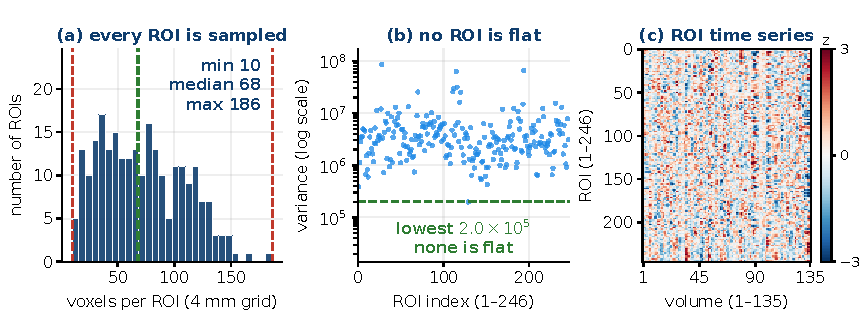
\includegraphics[width=\textwidth]{figures/atlas_roi_qc_slide.pdf}\\[4pt]
  \footnotesize\raggedright
  \textbf{246/246 ROIs are present in all 165 acquisitions:} no empty ROI (the smallest has 10 voxels),
  no zero-variance time series, no NaN or Inf. Every scan gives the same $135\times246$ matrix.\\[2pt]
  {\scriptsize (a): the atlas on the 4\,mm grid. (b), (c): one representative CN scan; (c) is z-scored
  per ROI for display.}
\end{frame}

% B5. 246 regions as connectivity nodes (for questions)
\begin{frame}{Backup: 246 Regions as Connectivity Nodes}
  \centering
  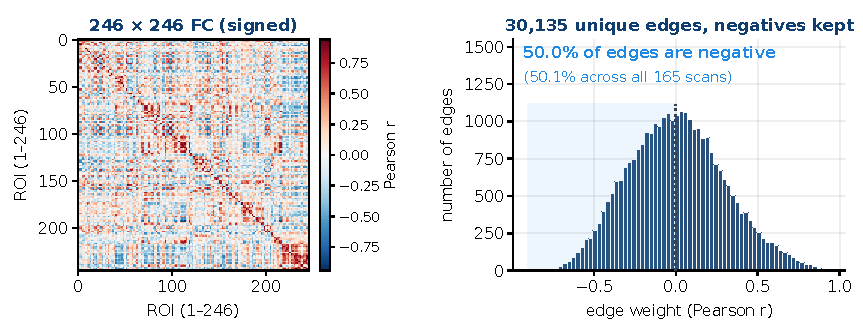
\includegraphics[width=\textwidth]{figures/atlas_fc_slide.pdf}\\[3pt]
  \footnotesize\raggedright
  \textbf{Signed and unthresholded:} all 30{,}135 unique edges are kept for each of the 165 acquisitions.
  About half are negative (50.1\,\% over the 165 scans; per-scan range 45.6--53.1\,\%), as expected after
  global signal regression, which is part of the 27-regressor design and centres the values near zero.\\[1pt]
  {\scriptsize Matrix and histogram: one representative CN scan.}
\end{frame}

% B6. Why 246 regions? (for questions)
\begin{frame}{Backup: Why 246 Regions?}
  \centering
  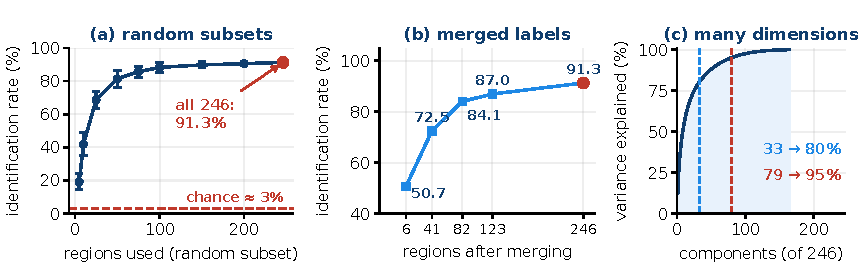
\includegraphics[width=\textwidth]{figures/findings_granularity.pdf}\\[2pt]
  \footnotesize\raggedright
  Closest-match identification (mALFF; 69 scans, 31 people; no stage label): merging consecutive atlas labels loses
  information at every step, but returns flatten (a random 100 regions: 88.3\,\%; all 246: \textbf{91.3\,\%}).
  Two regions share only about 4\,\% of their variance (165 scans).\par
  \vspace{0.15cm}
  \begin{block}{}
    \footnotesize Finer regions keep information that coarser versions of the same data lose. It does not show that
    246 is optimal for staging disease: only the trained model can test that.
  \end{block}
\end{frame}

% B7. Technology stack
\begin{frame}{Backup: Technology Stack}
  \small
  \begin{columns}[T,onlytextwidth]
    \column{0.52\textwidth}
      \begin{block}{Used so far (data foundation)}
        \footnotesize
        \begin{itemize}
          \item Python 3.12.3, NumPy, SciPy, pandas
          \item NiBabel 5.4.2, Nilearn 0.14.1
          \item ANTsPy 0.6.3 (registration), TemplateFlow 25.1.2
          \item FreeSurfer 7.4.1 (FS-FAST motion correction)
          \item WSL2 (Ubuntu) on Windows 11; Git
        \end{itemize}
      \end{block}
    \column{0.46\textwidth}
      \begin{block}{Planned (not yet used)}
        \footnotesize
        \begin{itemize}
          \item PyTorch, GPyTorch (model, Bayesian layers)
          \item Streamlit (Module 6 dashboard)
          \item Hardware per Review I: Intel Core i7, 32\,GB RAM, RTX 4060 (8\,GB)
        \end{itemize}
      \end{block}
  \end{columns}
  \vspace{0.2cm}
  {\footnotesize Dataset: ADNI via LONI. Versions are those recorded in each acquisition's provenance file.}
\end{frame}


% B8. Phase 2 details: the Meta-Bayesian model in plain words (design only)
\begin{frame}{The Meta-Bayesian Model in Plain Words (Design)}
  \centering
  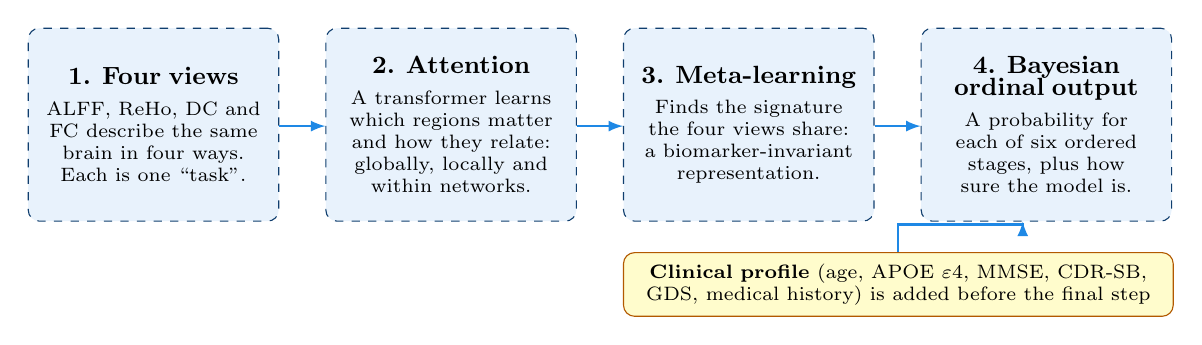
\begin{tikzpicture}[>=latex,
      card/.style={draw=UniversityBlue,dashed,rounded corners,fill=LightBlue,text width=2.9cm,
                   minimum height=2.45cm,align=center,font=\scriptsize,inner sep=4pt,anchor=north west},
      ar/.style={->,thick,draw=AccentBlue}]
    \node[card] (c1) at (0,0)    {{\small\bfseries 1. Four views}\\[3pt] ALFF, ReHo, DC and FC describe the same brain in four ways. Each is one ``task''.};
    \node[card] (c2) at (3.78,0) {{\small\bfseries 2. Attention}\\[3pt] A transformer learns which regions matter and how they relate: globally, locally and within networks.};
    \node[card] (c3) at (7.56,0) {{\small\bfseries 3. Meta-learning}\\[3pt] Finds the signature the four views share: a biomarker-invariant representation.};
    \node[card] (c4) at (11.34,0) {{\small\bfseries 4. Bayesian ordinal output}\\[3pt] A probability for each of six ordered stages, plus how sure the model is.};
    \foreach \a/\b in {c1/c2,c2/c3,c3/c4} \draw[ar] (\a.east |- 0,-1.25) -- (\b.west |- 0,-1.25);
    \node[draw=orange!70!black,fill=yellow!20,rounded corners,font=\scriptsize,text width=6.7cm,
          align=center,inner sep=4pt,anchor=north west] (cl) at (7.56,-2.85)
      {\textbf{Clinical profile} (age, APOE $\varepsilon$4, MMSE, CDR-SB, GDS, medical history) is added before the final step};
    \draw[ar] (cl.north) -- ++(0,0.35) -| ([xshift=-0.3cm]c4.south);
  \end{tikzpicture}
  \vspace{0.1cm}

  \begin{itemize}
    \item \textbf{Ordinal:} CN$\to$AD is a progression, so confusing neighbouring stages is a smaller error than confusing distant ones.
    \item \textbf{Bayesian:} borderline subjects get a wide uncertainty instead of a falsely confident label.
  \end{itemize}
  \begin{alertblock}{}
    \small \textbf{Design only.} Nothing is trained; no accuracy, calibration or attention result exists.
  \end{alertblock}
\end{frame}

% B9. Phase 2 details: Core Algorithm B (design only)
\begin{frame}{Core Algorithm B: Meta-Bayesian Pipeline (Design, Not Implemented)}
  \centering
  {\small \alert{Design only: nothing is trained and no result exists.}}\par
  \resizebox{0.84\textwidth}{!}{%
  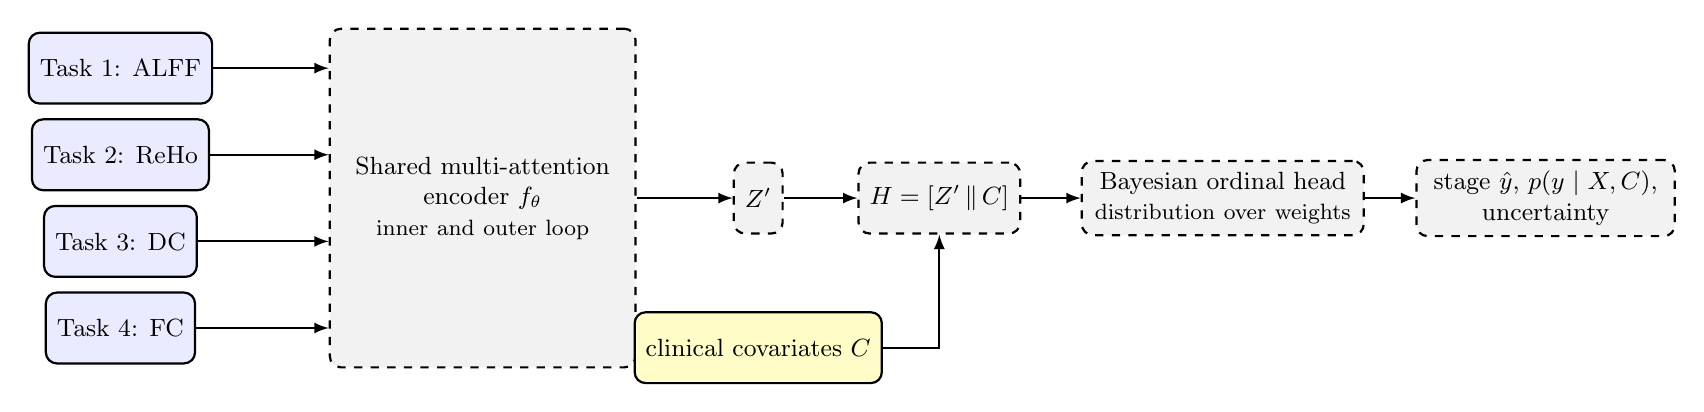
\begin{tikzpicture}[font=\small,>=latex]
    \tikzset{b/.style={rounded corners,thick,draw,align=center,minimum height=0.9cm,inner sep=4pt},
             ar/.style={->,thick}}
    \node[b,fill=blue!8] (t1) at (0,1.65) {Task 1: ALFF};
    \node[b,fill=blue!8] (t2) at (0,0.55) {Task 2: ReHo};
    \node[b,fill=blue!8] (t3) at (0,-0.55) {Task 3: DC};
    \node[b,fill=blue!8] (t4) at (0,-1.65) {Task 4: FC};
    \node[b,fill=gray!10,dashed,text width=3.6cm,minimum height=4.3cm] (enc) at (4.6,0) {Shared multi-attention\\encoder $f_\theta$\\{\footnotesize inner and outer loop}};
    \node[b,fill=gray!10,dashed] (z) at (8.1,0) {$Z'$};
    \node[b,fill=yellow!22] (c) at (8.1,-1.9) {clinical covariates $C$};
    \node[b,fill=gray!10,dashed] (h) at (10.4,0) {$H=[Z'\,\|\,C]$};
    \node[b,fill=gray!10,dashed,text width=3.3cm] (head) at (14.0,0) {Bayesian ordinal head\\{\footnotesize distribution over weights}};
    \node[b,fill=gray!10,dashed,text width=3.0cm] (out) at (18.1,0) {stage $\hat y$, $p(y\mid X,C)$,\\uncertainty};
    \foreach \t in {t1,t2,t3,t4} \draw[ar] (\t.east) -- (enc.west |- \t.east);
    \draw[ar] (enc) -- (z); \draw[ar] (z) -- (h); \draw[ar] (c.east) -| (h.south);
    \draw[ar] (h) -- (head); \draw[ar] (head) -- (out);
  \end{tikzpicture}}
  \vspace{-0.1cm}

  \begin{columns}[T,onlytextwidth]
    \column{0.49\textwidth}
      \begin{block}{MAML update over biomarkers}
        \scriptsize
        \vspace{-4pt}
        \begin{align*}
          \theta'_b &= \theta-\alpha\,\nabla_\theta\mathcal{L}^{\mathrm{sup}}_b(\theta)\\
          \theta &\leftarrow \theta-\beta\,\nabla_\theta\sum_{b}\mathcal{L}^{\mathrm{qry}}_b(\theta'_b)
        \end{align*}
        \vspace{-8pt}
      \end{block}
    \column{0.49\textwidth}
      \begin{block}{Ordinal head (cumulative link)}
        \scriptsize
        \vspace{-4pt}
        \begin{equation*}
          P(y\le k\mid H,w)=\sigma\bigl(\tau_k-g_w(H)\bigr),\quad \tau_0<\dots<\tau_4
        \end{equation*}
        \vspace{-8pt}
      \end{block}
  \end{columns}
  {\scriptsize Support and query sets are subject-disjoint, within training folds.
  Uncertainty = predictive entropy over $S$ weight samples.}
\end{frame}

% B10. First Review - Queries and Answers (last slide)
\begin{frame}{First Review - Queries and Answers}
  \small
  \begin{tabularx}{\textwidth}{>{\raggedright\arraybackslash}p{3.9cm}>{\raggedright\arraybackslash}X>{\raggedright\arraybackslash}p{2.8cm}}
    \toprule
    \textbf{Panel comment} & \textbf{Response} & \textbf{Detail in} \\
    \midrule
    Need more clarity on the \textbf{dataset (biomarkers)} &
    175 audited, 165 preprocessed, 127 subjects. Four biomarkers on 246 regions. &
    Dataset and biomarker slides; report \S6.1 \\[4pt]
    Need more clarity on the \textbf{Meta-Bayesian framework} &
    ``Meta'': biomarkers as tasks. ``Bayesian'': ordinal head with uncertainty.
    \alert{Design only.} &
    Phase 2 slides (at the end); report \S4.5 \\[4pt]
    Need more clarity on the \textbf{comorbidity data} &
    Seven covariates, listed on the covariates slide. Cleaned table for 127 subjects; the LMCI group has APOE only. &
    Covariates slide; report \S4.5 \\
    \bottomrule
  \end{tabularx}
\end{frame}

\end{document}
